\chapter{Procedure}

\section{AC Sweep/Noise Analysis}

\subsection{Theoretical Analysis}

\begin{figure}[h]
    \centering
    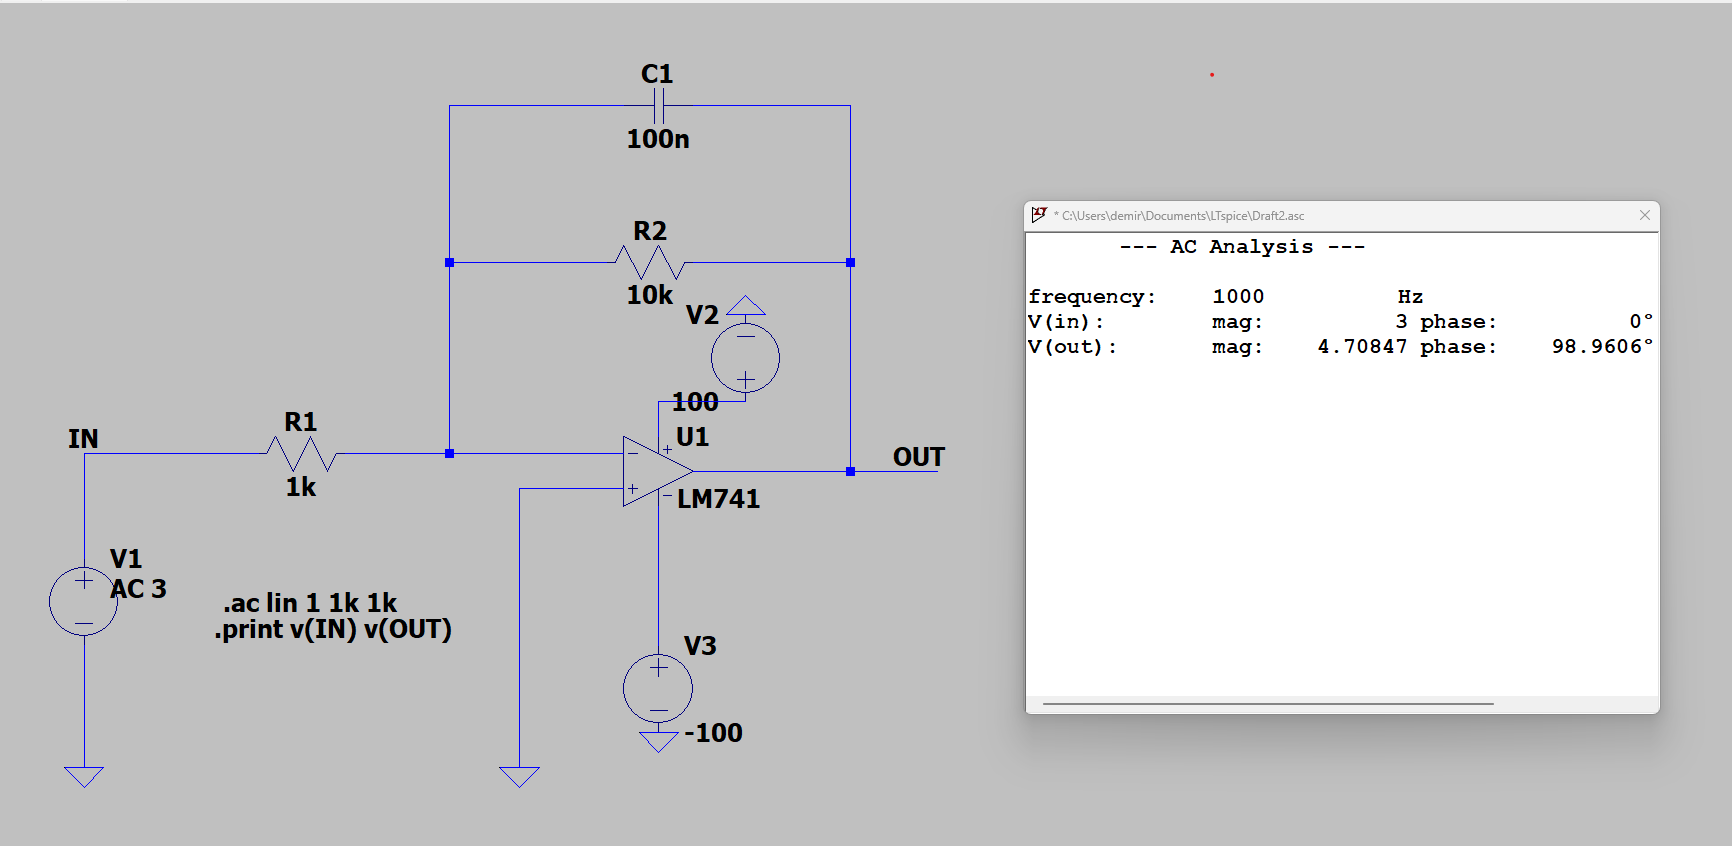
\includegraphics[width=0.6\textwidth]{assets/p1-1k.png}
    \caption{AC Analysis Circuit}
    \label{fig:ac-analysis-circuit}
|\end{figure}

\begin{table}[h]
    \centering
    \begin{tabular}{llll}
    \cline{1-2}
    \multicolumn{1}{|l|}{Frequency} & \multicolumn{1}{l|}{1kHz} &             &                              \\ \hline
    \multicolumn{1}{|l|}{$V_{in}$}     & mag: 3                    & phase: $0^{\circ}$    & \multicolumn{1}{l|}{} \\ \hline
    \multicolumn{1}{|l|}{$V_{out}$}    & mag: 4.70847               & phase: $98.96^{\circ}$ & \multicolumn{1}{l|}{} \\ \hline
                                    &                           &             &                             
    \end{tabular}
    \caption{AC Analysis Results}
    \label{tab:ac-sweep-analysis-results}
\end{table}

From the results, we can make these observations:

\begin{itemize}
    \item \textbf{Magnitude:} The gain of the circuit is approximately $1.57$ at $1kHz$. 
    \item \textbf{Phase:} The input signal has a phase of $0^{\circ}$, while the output signal exhibits a phase shift of $98.96^{\circ}$. This significant phase shift is typical in op-amp circuits operating at high frequencies. As the frequency increases, op-amps tend to introduce phase shifts due to internal capacitances and feedback delays. A shift of approximately 99° suggests that the circuit is approaching the higher end of the op-amp’s bandwidth, which leads to a lag in the output signal.
\end{itemize}

\newpage
\thispagestyle{plain}

\subsection{Experimental Analysis}

To verify the theoretical results, we built the same circuit on a breadboard and measured the input and output voltages using an oscilloscope.

\begin{figure}[h]
    \centering
    \begin{minipage}{.5\textwidth}
        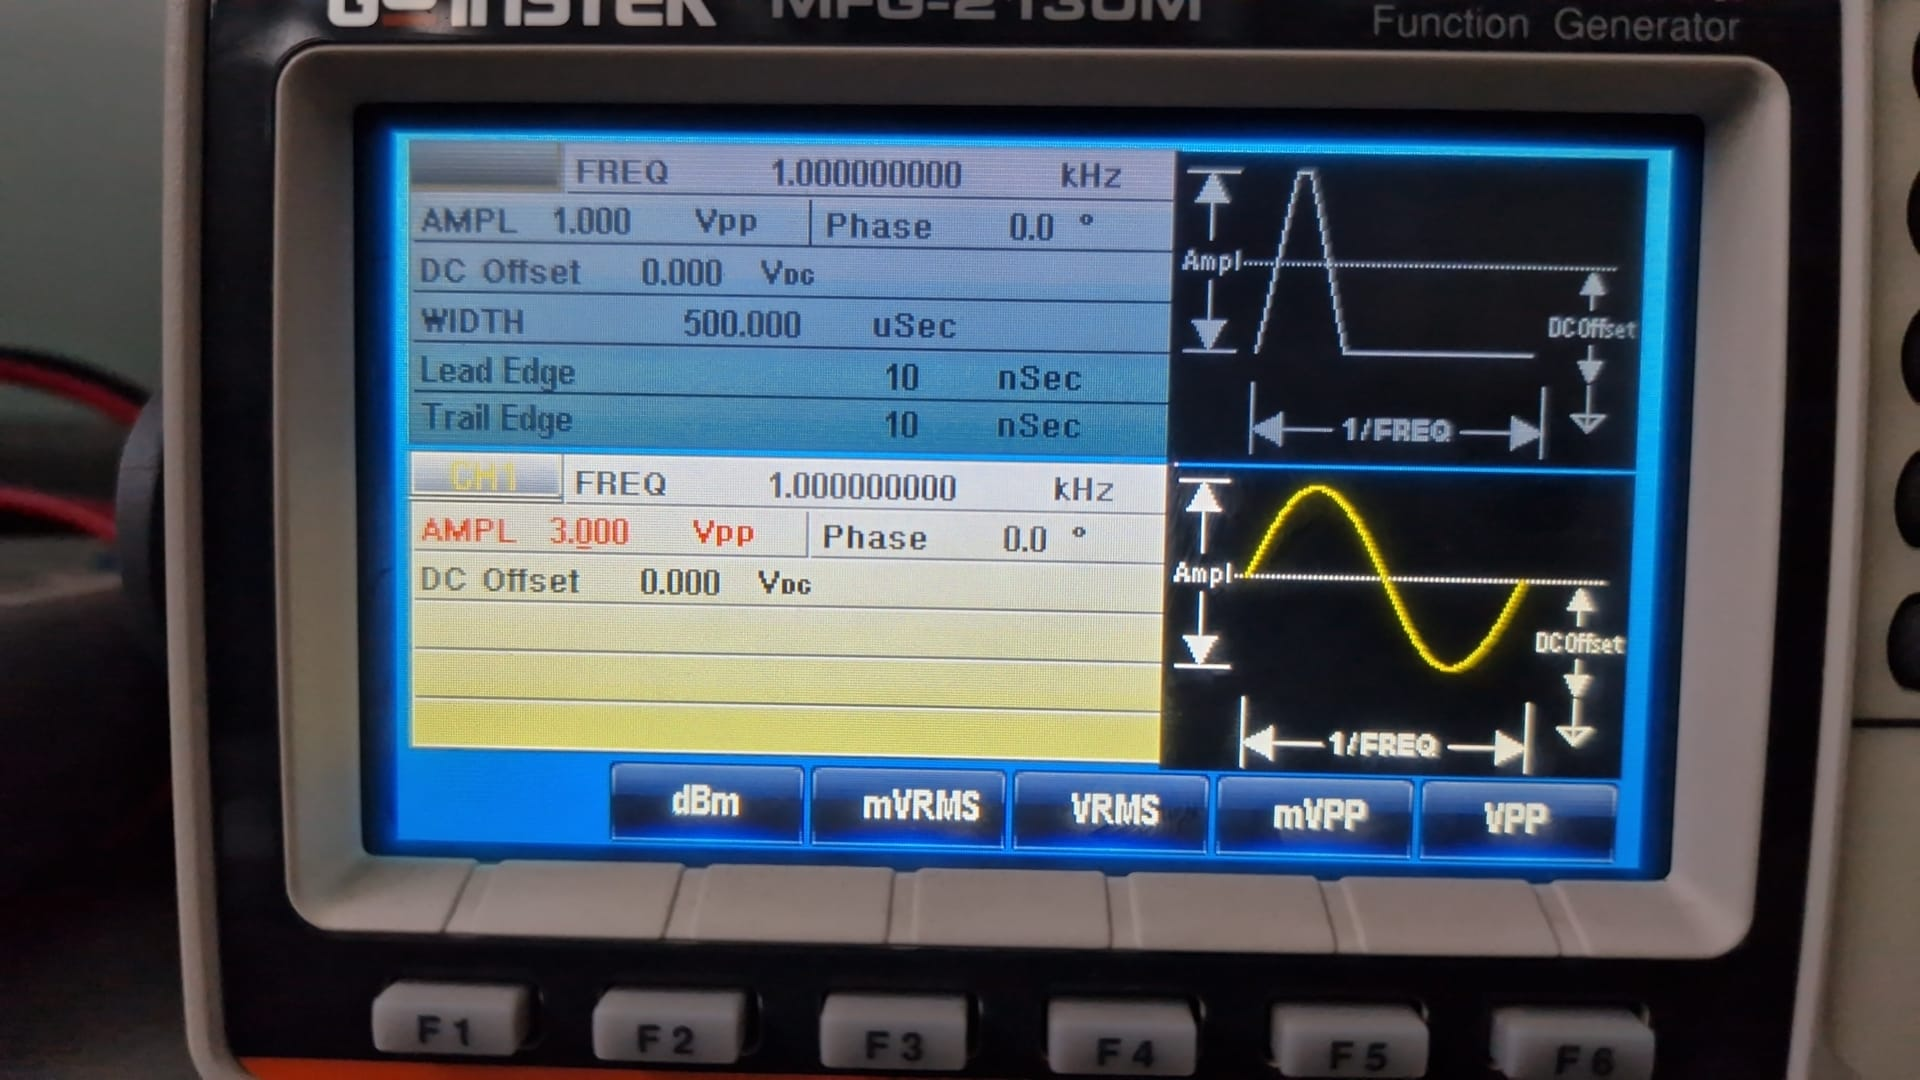
\includegraphics[width=1\linewidth]{assets/p1-result-experimet-signal.png}
        \caption{$3V_ {pp}~@~1kHz$ Input signal}
        \label{fig:p1-result-experiment-signal}
    \end{minipage}%
    \begin{minipage}{.5\textwidth}
        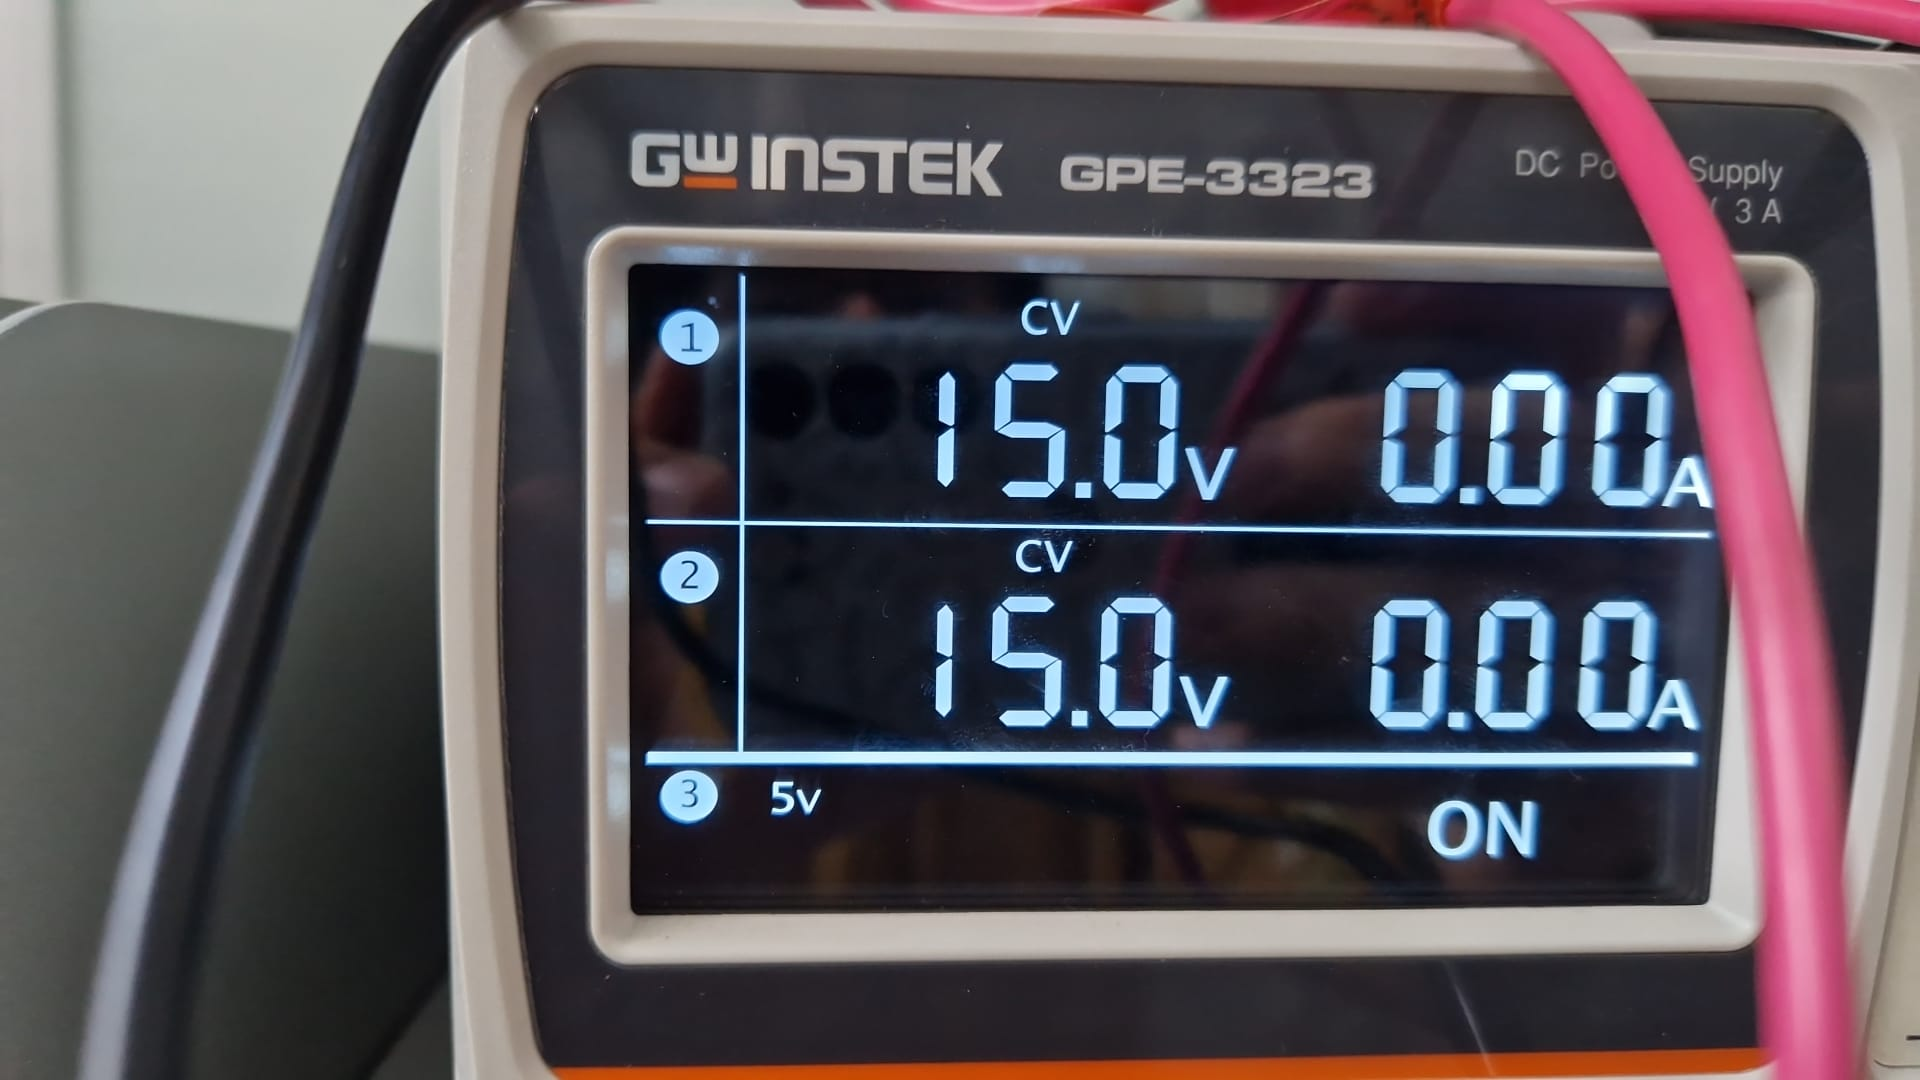
\includegraphics[width=1\linewidth]{assets/pm-15v.png}
        \caption{15V DC Power Supply}
        \label{fig:experiment-15v-power}
    \end{minipage}
\end{figure}

\begin{figure}[h]
    \centering
    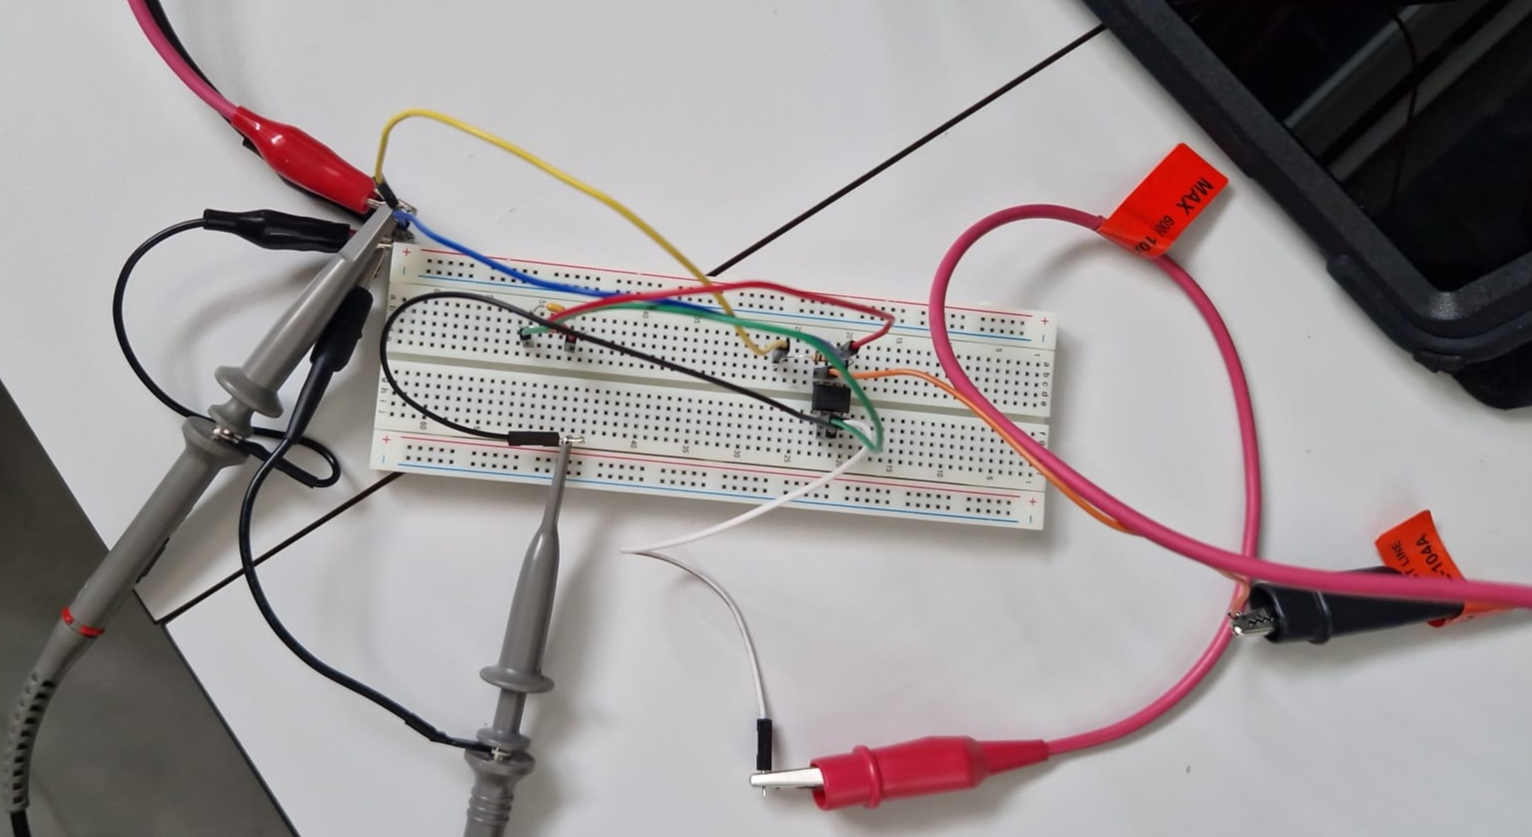
\includegraphics[width=1\textwidth]{assets/p1-2-circuit.png}
    \caption{Experiment Circuit}
    \label{fig:p1-2-circuit}
|\end{figure}

According to theoretical analysis, the output voltage should be $3\times 1.57 = 4.71V$

\newpage
\thispagestyle{plain}

\begin{figure}[h]
    \centering
    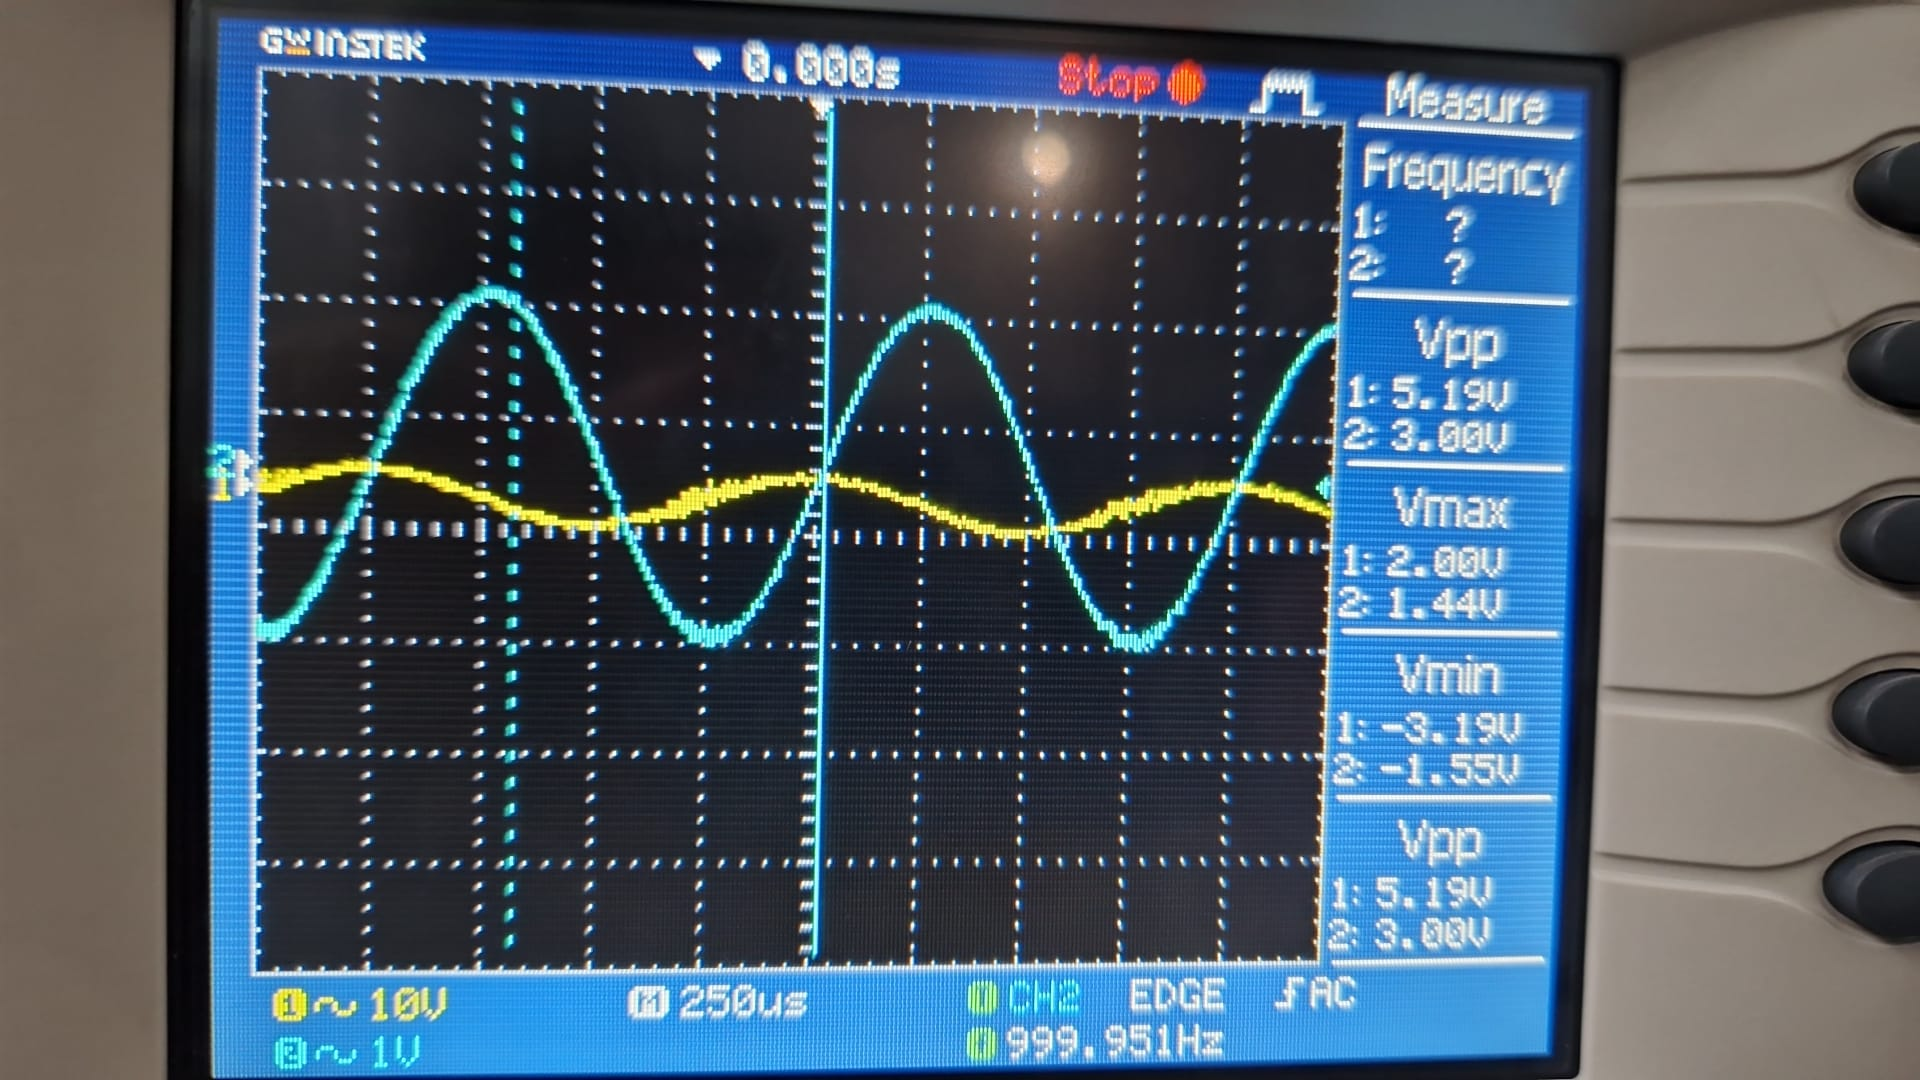
\includegraphics[width=1\textwidth]{assets/p1-result-experimet-ossiloscope.png}
    \caption{Experiment Result}
    \label{fig:p1-experiment-result}
|\end{figure}

But the oscilloscope reads $5.19V$ which means real gain is $\frac{5.19}{3} = 1.73$ which is approximately $10\%$ higher than the theoretical value. This can be due to the tolerances of the resistors used in the circuit and the op-amp itself.

Also used $110nF$ capacitor instead of $100nF$ capacitor in the experimental analysis due to the lack of $1nF$ capacitor. This can also cause a slight difference in the results.

\newpage{}
\thispagestyle{plain}

\section{Frequency Response Analysis}

\subsection{Theoretical Analysis}

\begin{figure}[h]
    \centering
    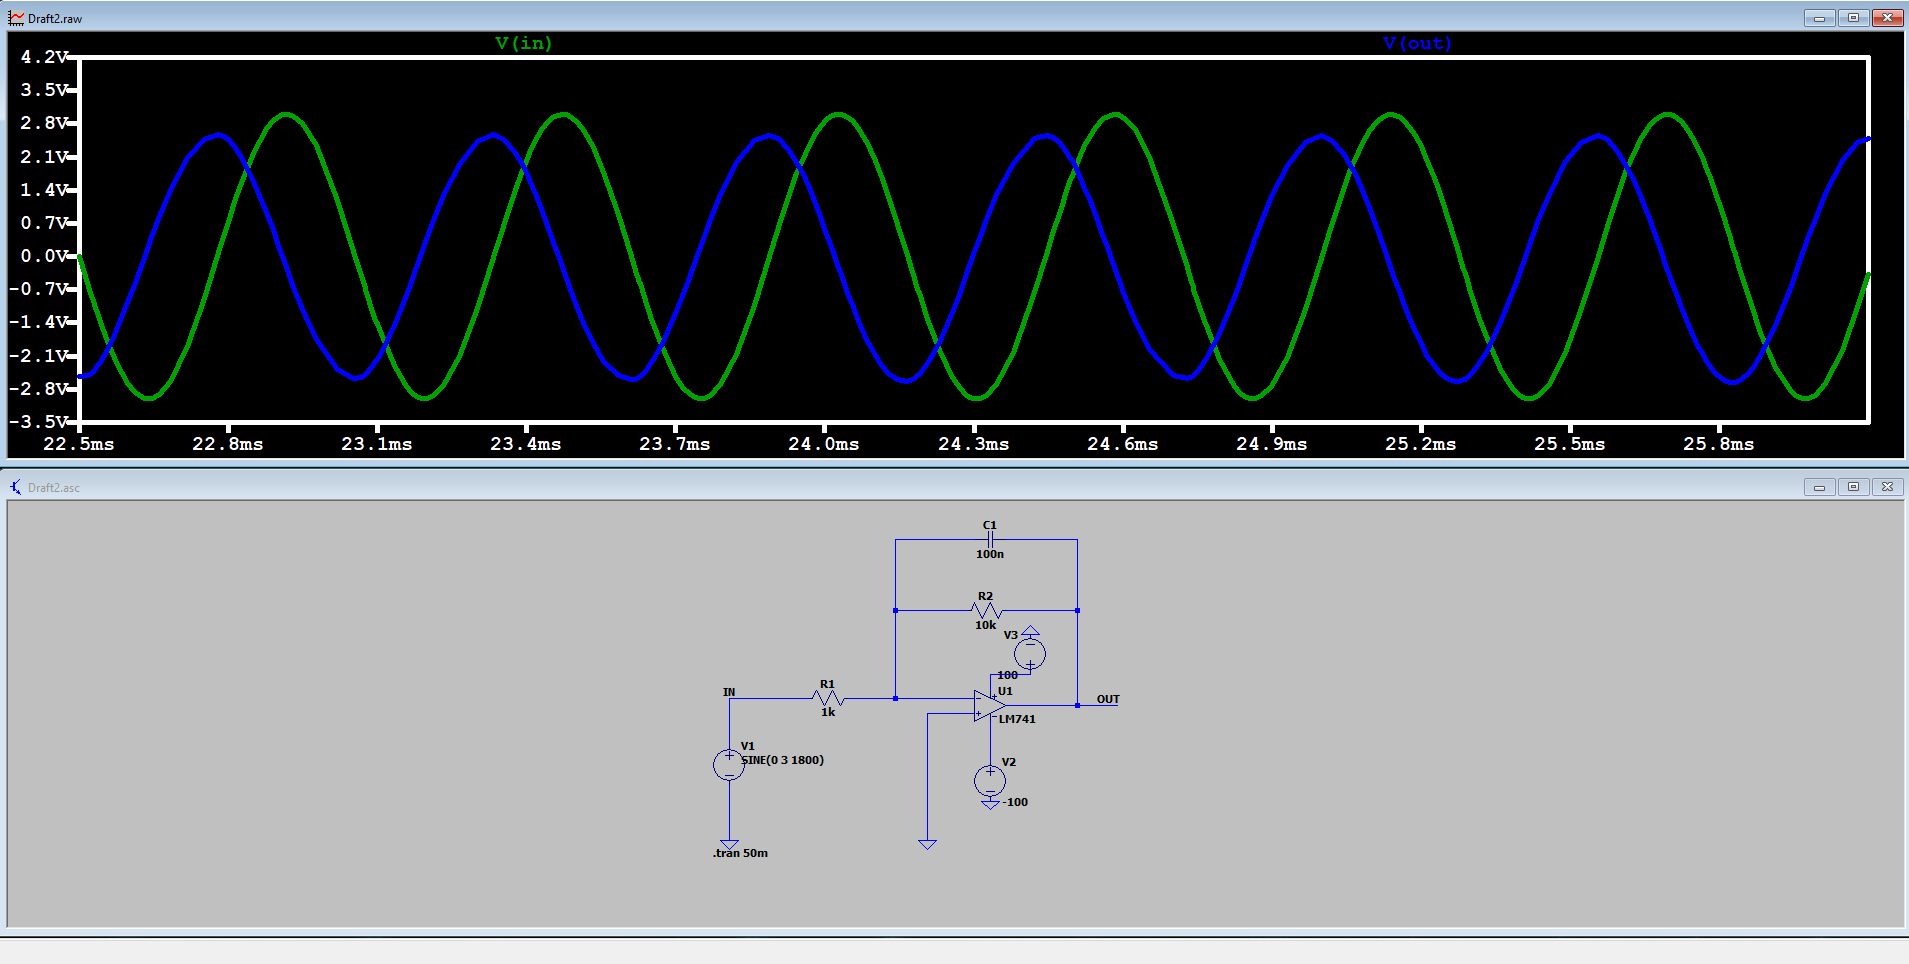
\includegraphics[width=0.8\textwidth]{assets/p2-1.8k.png}
    \caption{Frequency Response Analysis Circuit @ 1.8kHz}
    \label{fig:frequency-response-analysis-circuit-1.8k}
\end{figure}

\begin{figure}[h]
    \centering
    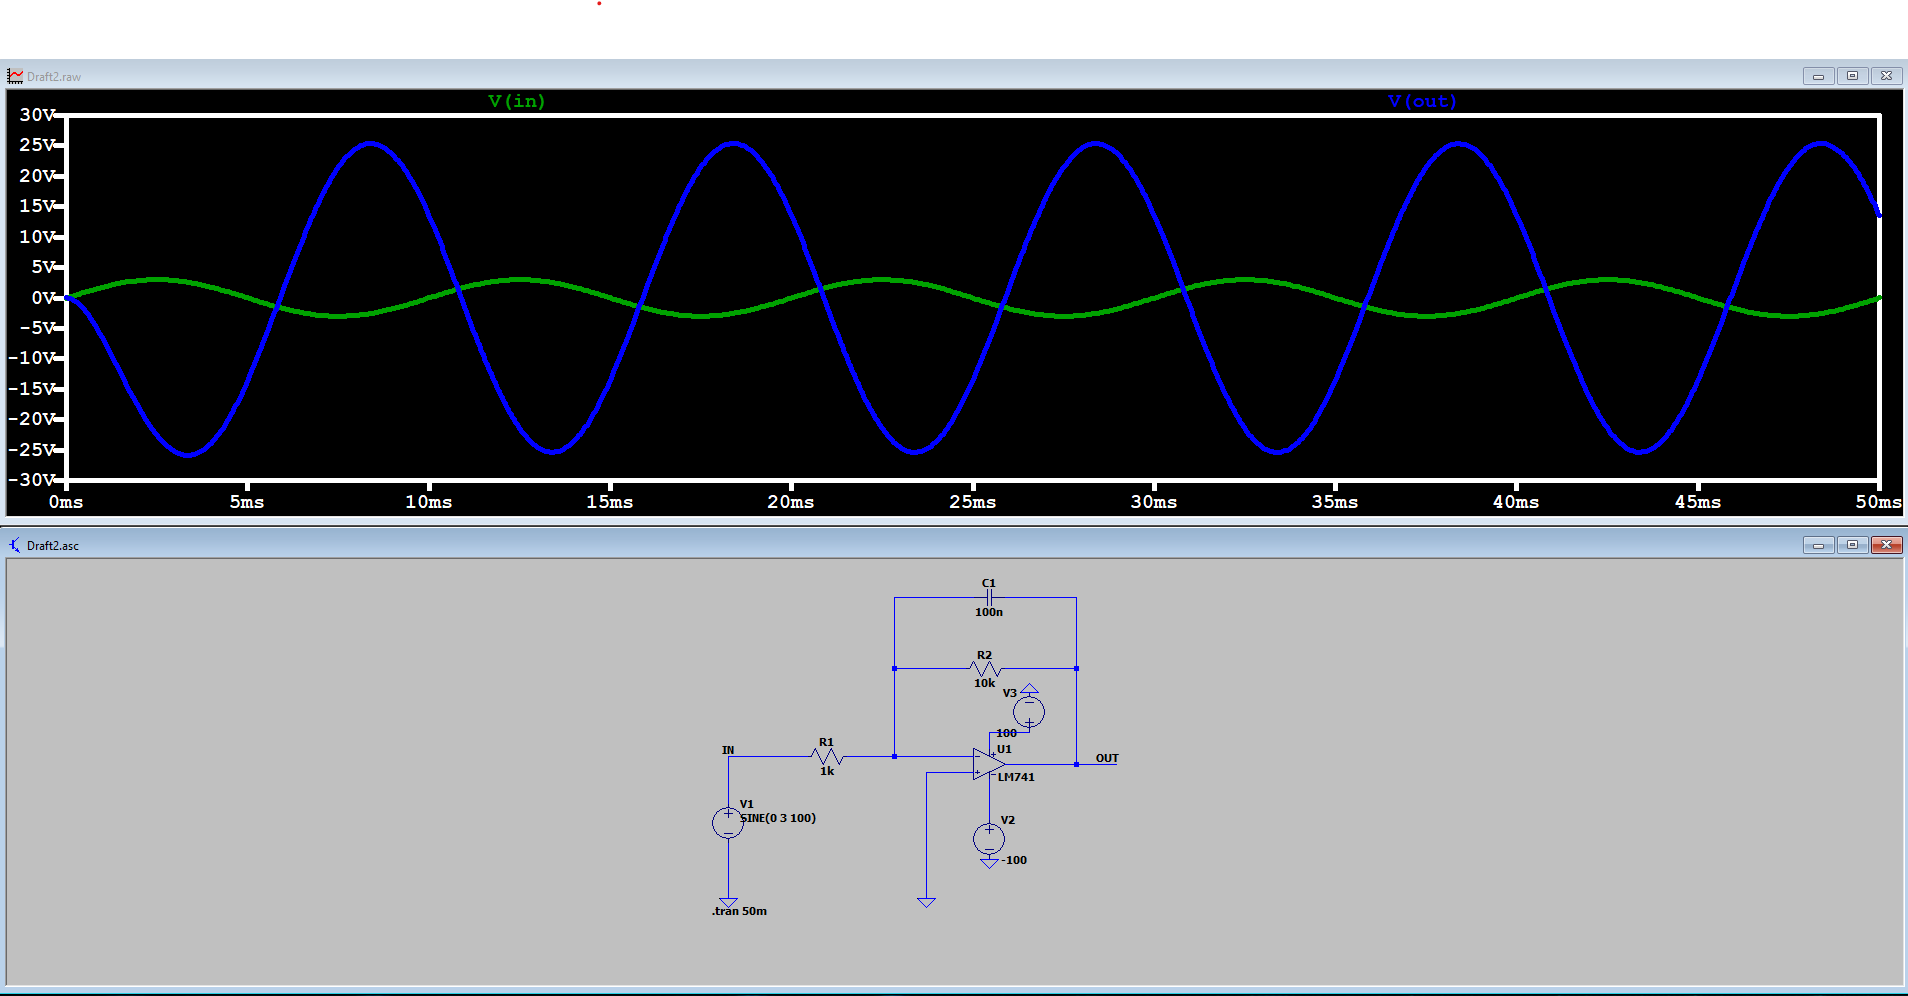
\includegraphics[width=0.8\textwidth]{assets/p2-100.png}
    \caption{Frequency Response Analysis Circuit @ 100Hz}
    \label{fig:frequency-response-analysis-circuit-100}
\end{figure}

At lower frequencies, op-amp behaves as expected. However, at higher frequencies, output starts to lag behing the input due to phase shifts, and the amplitude decreases, indicating a drop in gain as the op-amp bandwidth is exceeded.

\newpage
\thispagestyle{plain}

\subsection{Experimental Analysis}
To verify the theoretical results, we built the same circuit on a breadboard (Figure \ref{fig:p1-2-circuit}) and measured the input and output voltages using an oscilloscope.

\begin{figure}[h]
    \centering
    \begin{minipage}{.4\textwidth}
        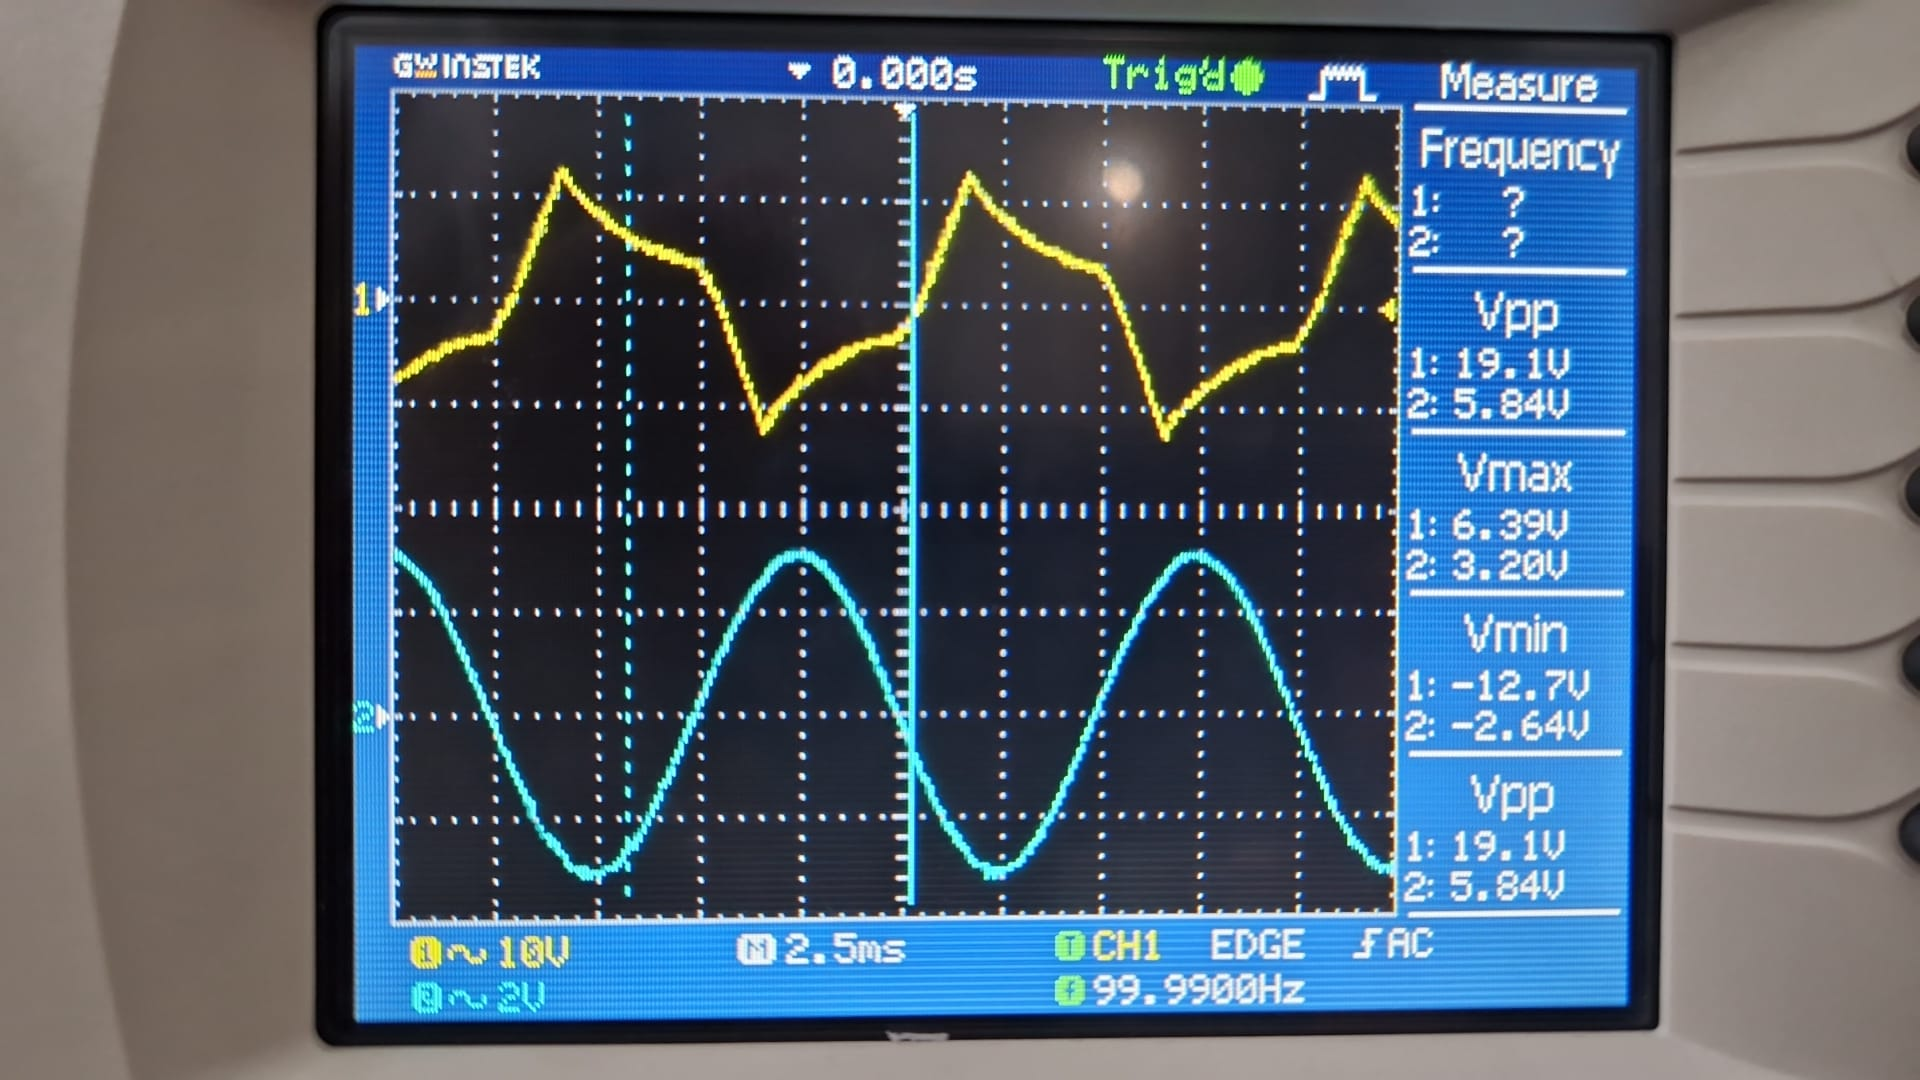
\includegraphics[width=1\linewidth]{assets/p2-exp-100.png}
        \caption{$100Hz$ Input signal}
        \label{fig:p2-exp-100}
    \end{minipage}%
    \begin{minipage}{.4\textwidth}
        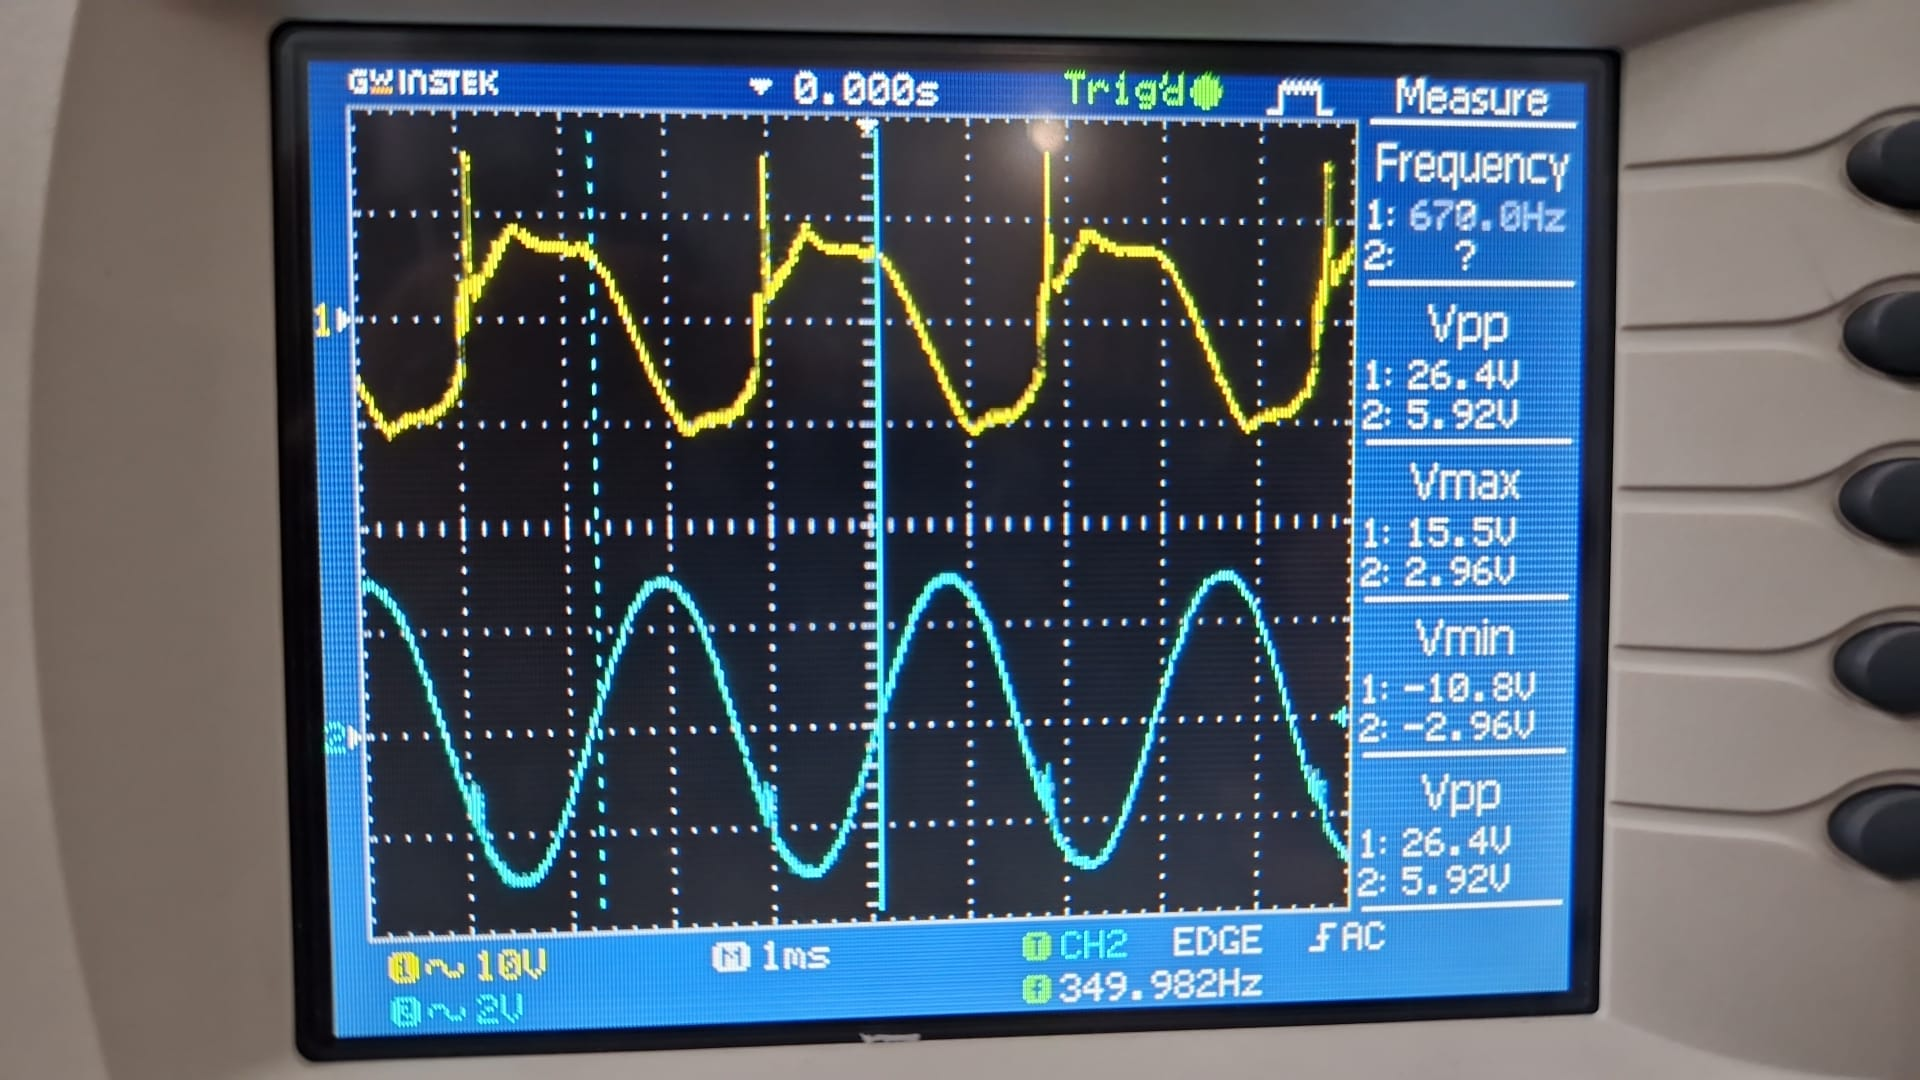
\includegraphics[width=1\linewidth]{assets/p2-exp-350.png}
        \caption{$350Hz$ Input signal}
        \label{fig:p2-exp-350}
    \end{minipage}
    \begin{minipage}{.4\textwidth}
        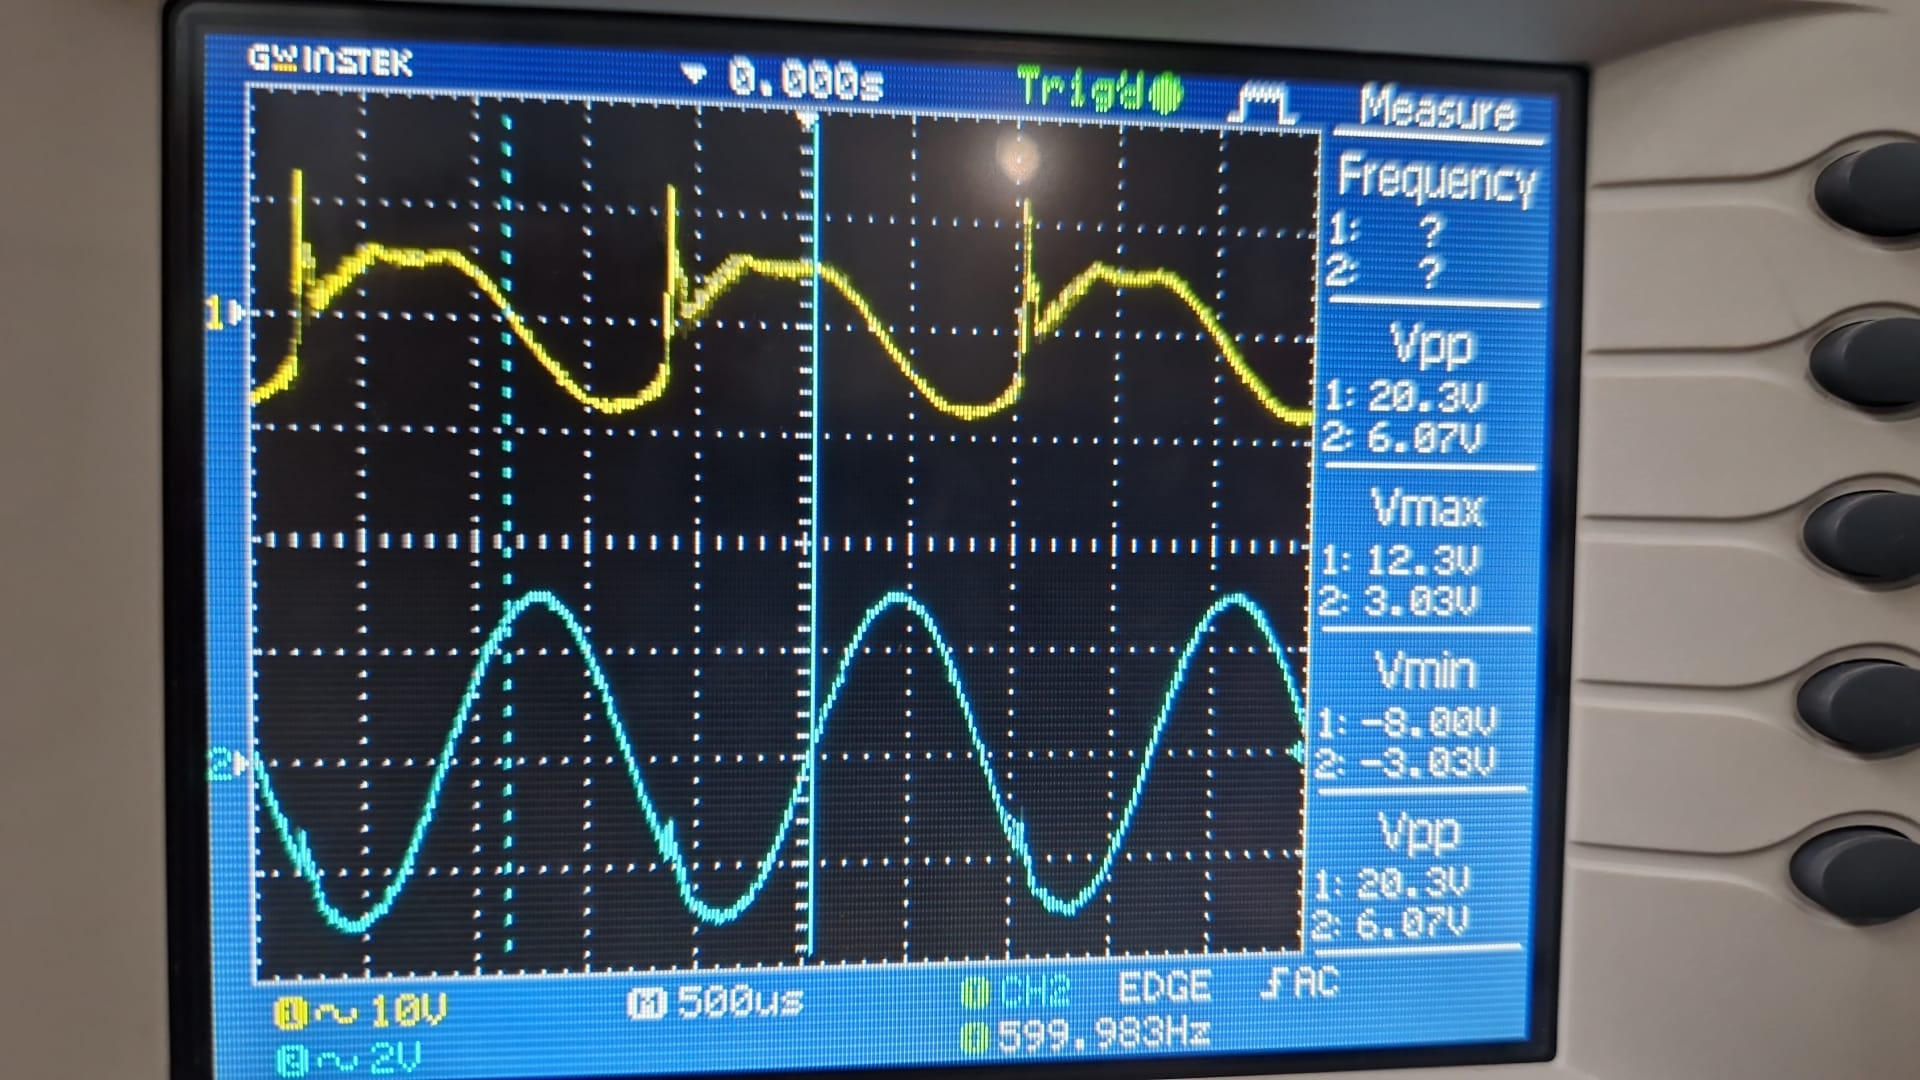
\includegraphics[width=1\linewidth]{assets/p2-exp-600.png}
        \caption{$600Hz$ Input signal}
        \label{fig:p2-exp-600}
    \end{minipage}%
    \begin{minipage}{.4\textwidth}
        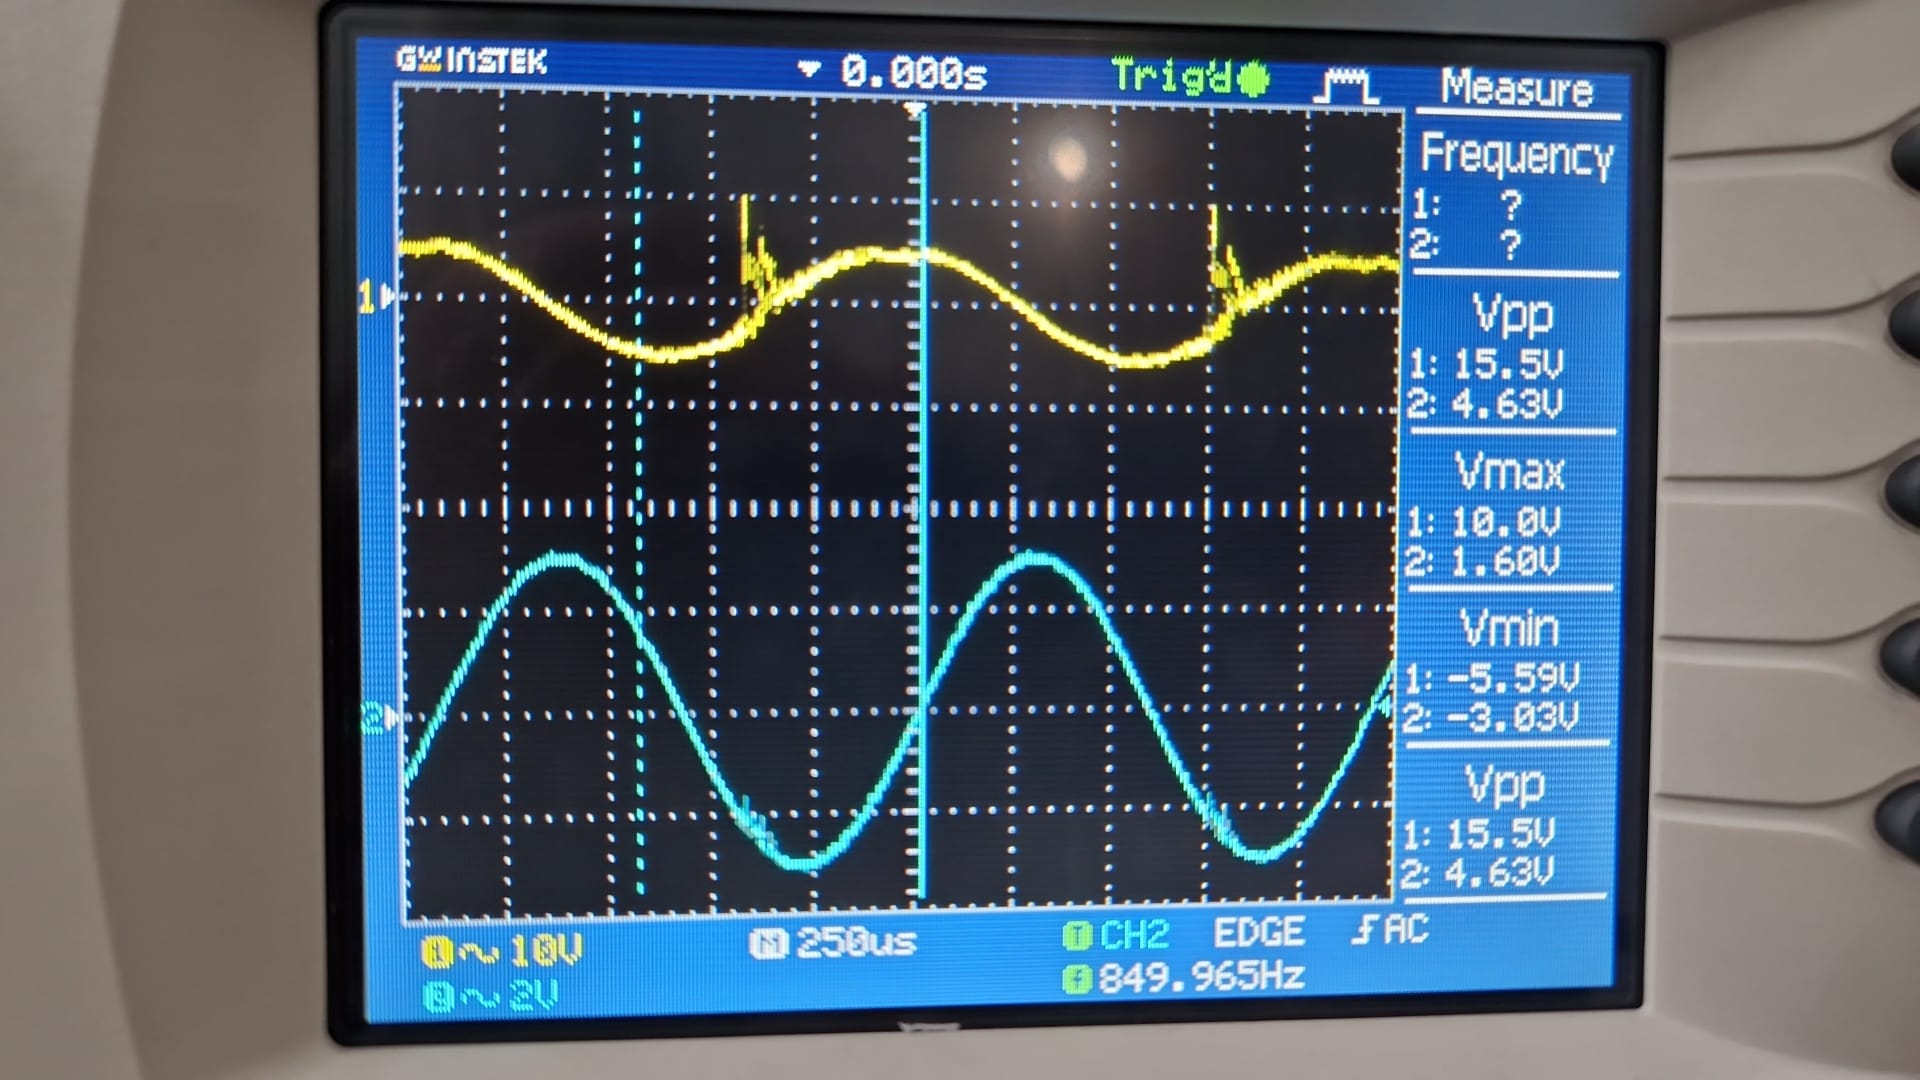
\includegraphics[width=1\linewidth]{assets/p2-exp-850.png}
        \caption{$850Hz$ Input signal}
        \label{fig:p2-exp-850}
    \end{minipage}
    \begin{minipage}{.4\textwidth}
        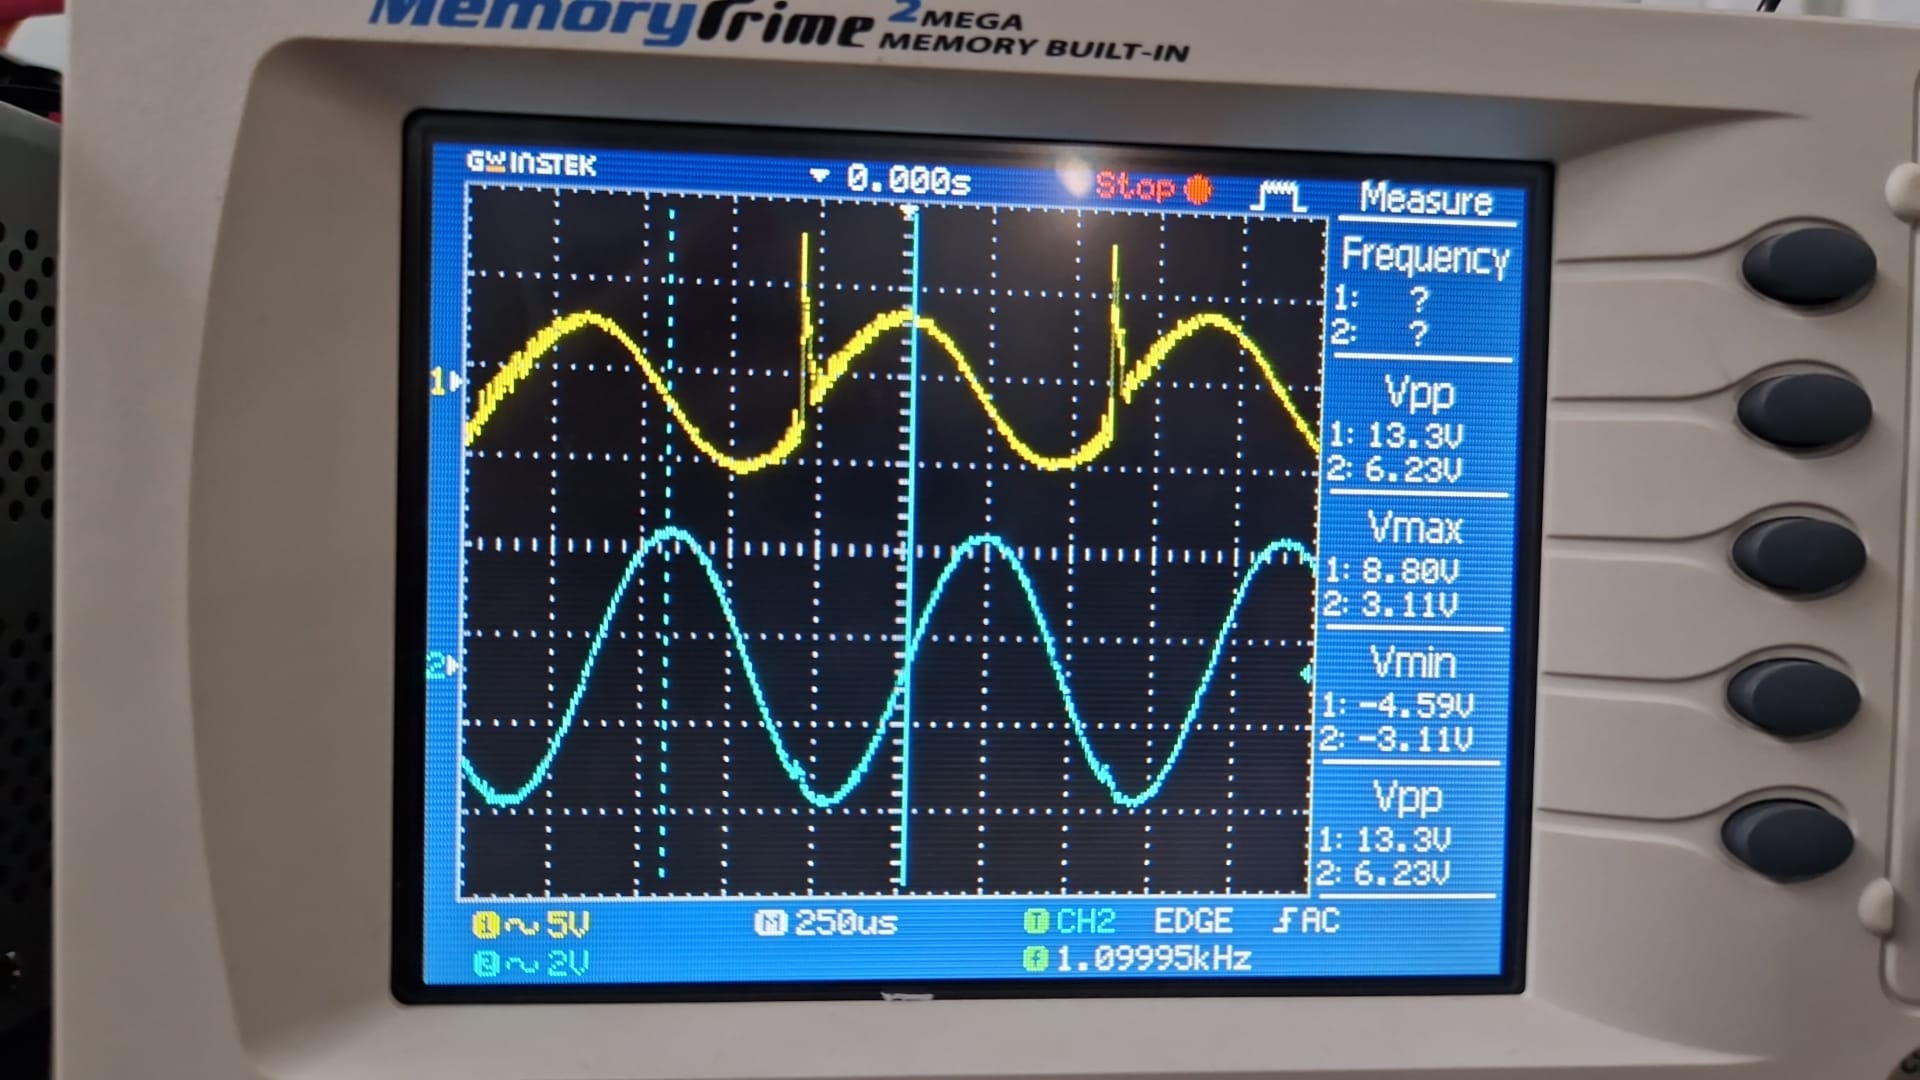
\includegraphics[width=1\linewidth]{assets/p2-exp-1.1.png}
        \caption{$1.1kHz$ Input signal}
        \label{fig:p2-exp-1.1}
    \end{minipage}%
    \begin{minipage}{.4\textwidth}
        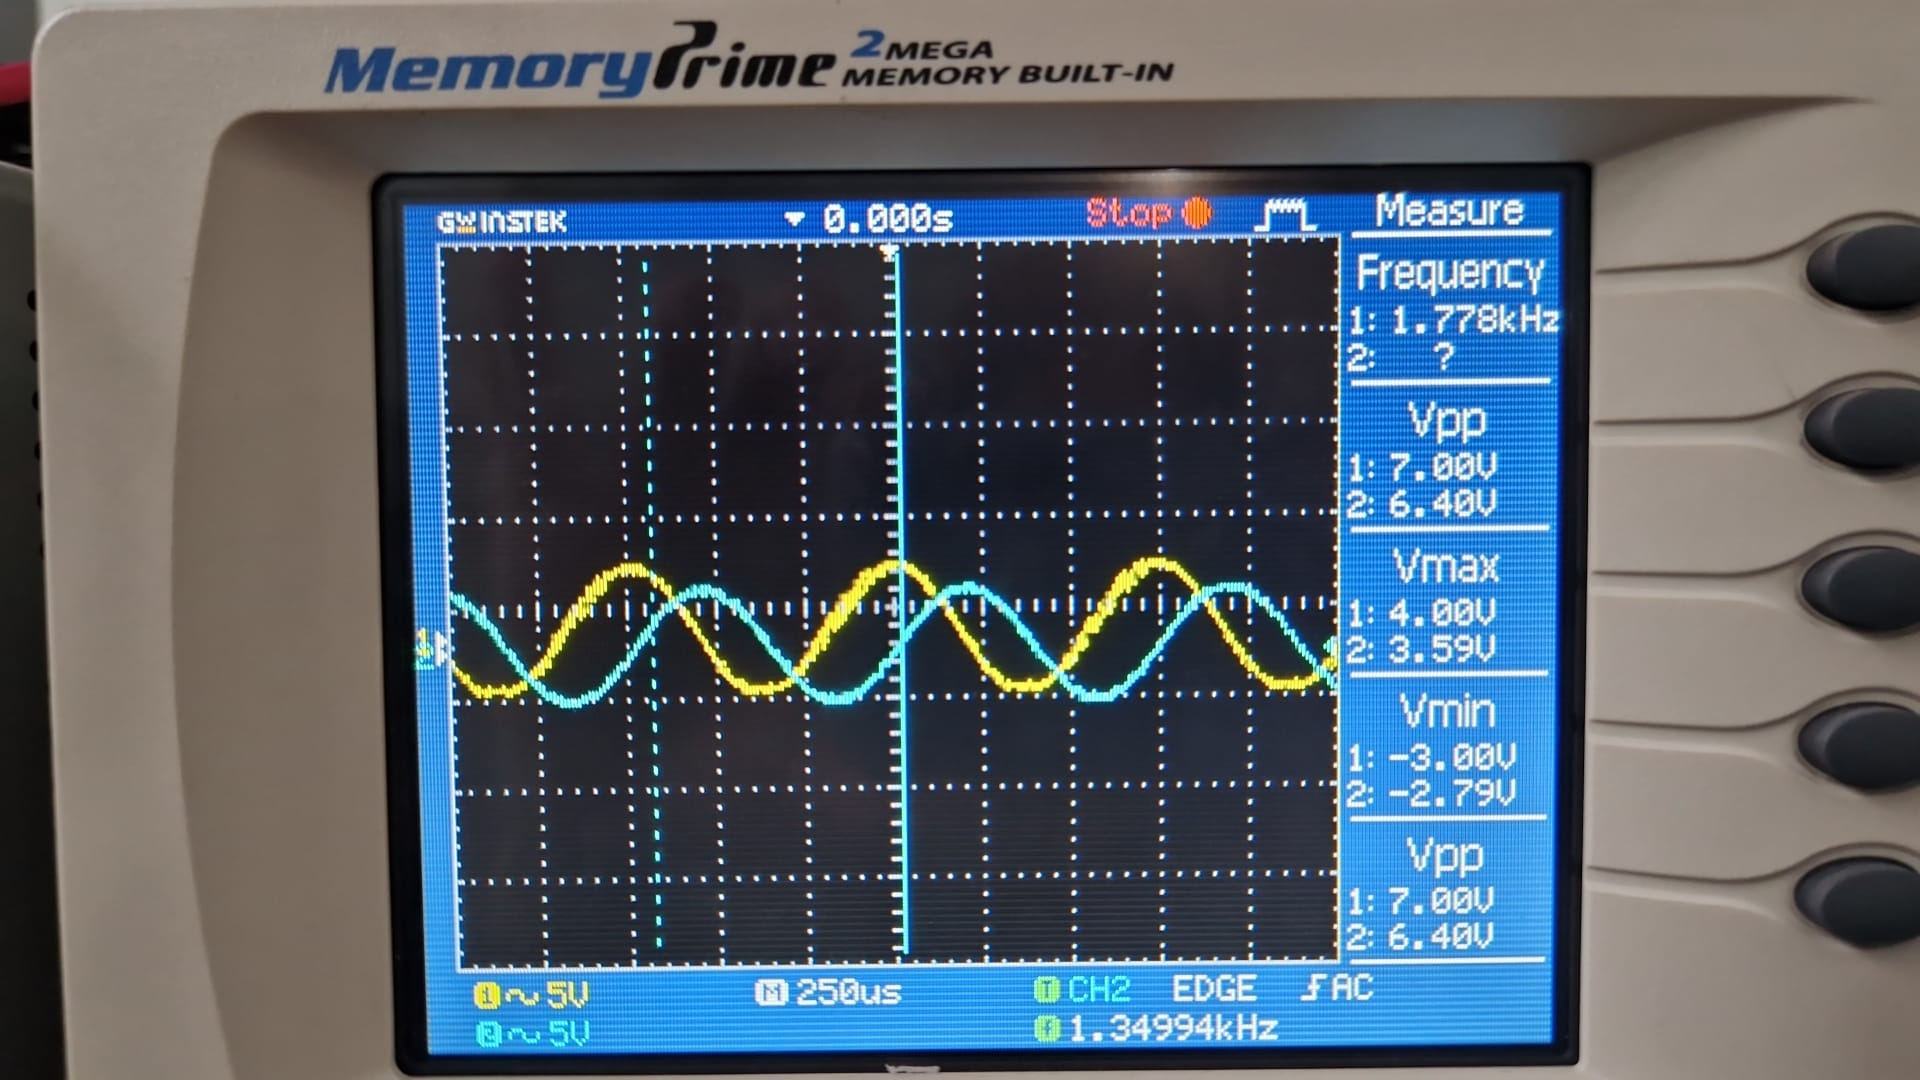
\includegraphics[width=1\linewidth]{assets/p2-exp-1.35.png}
        \caption{$1.35Hz$ Input signal}
        \label{fig:p2-exp-1.35}
    \end{minipage}
    \begin{minipage}{.4\textwidth}
        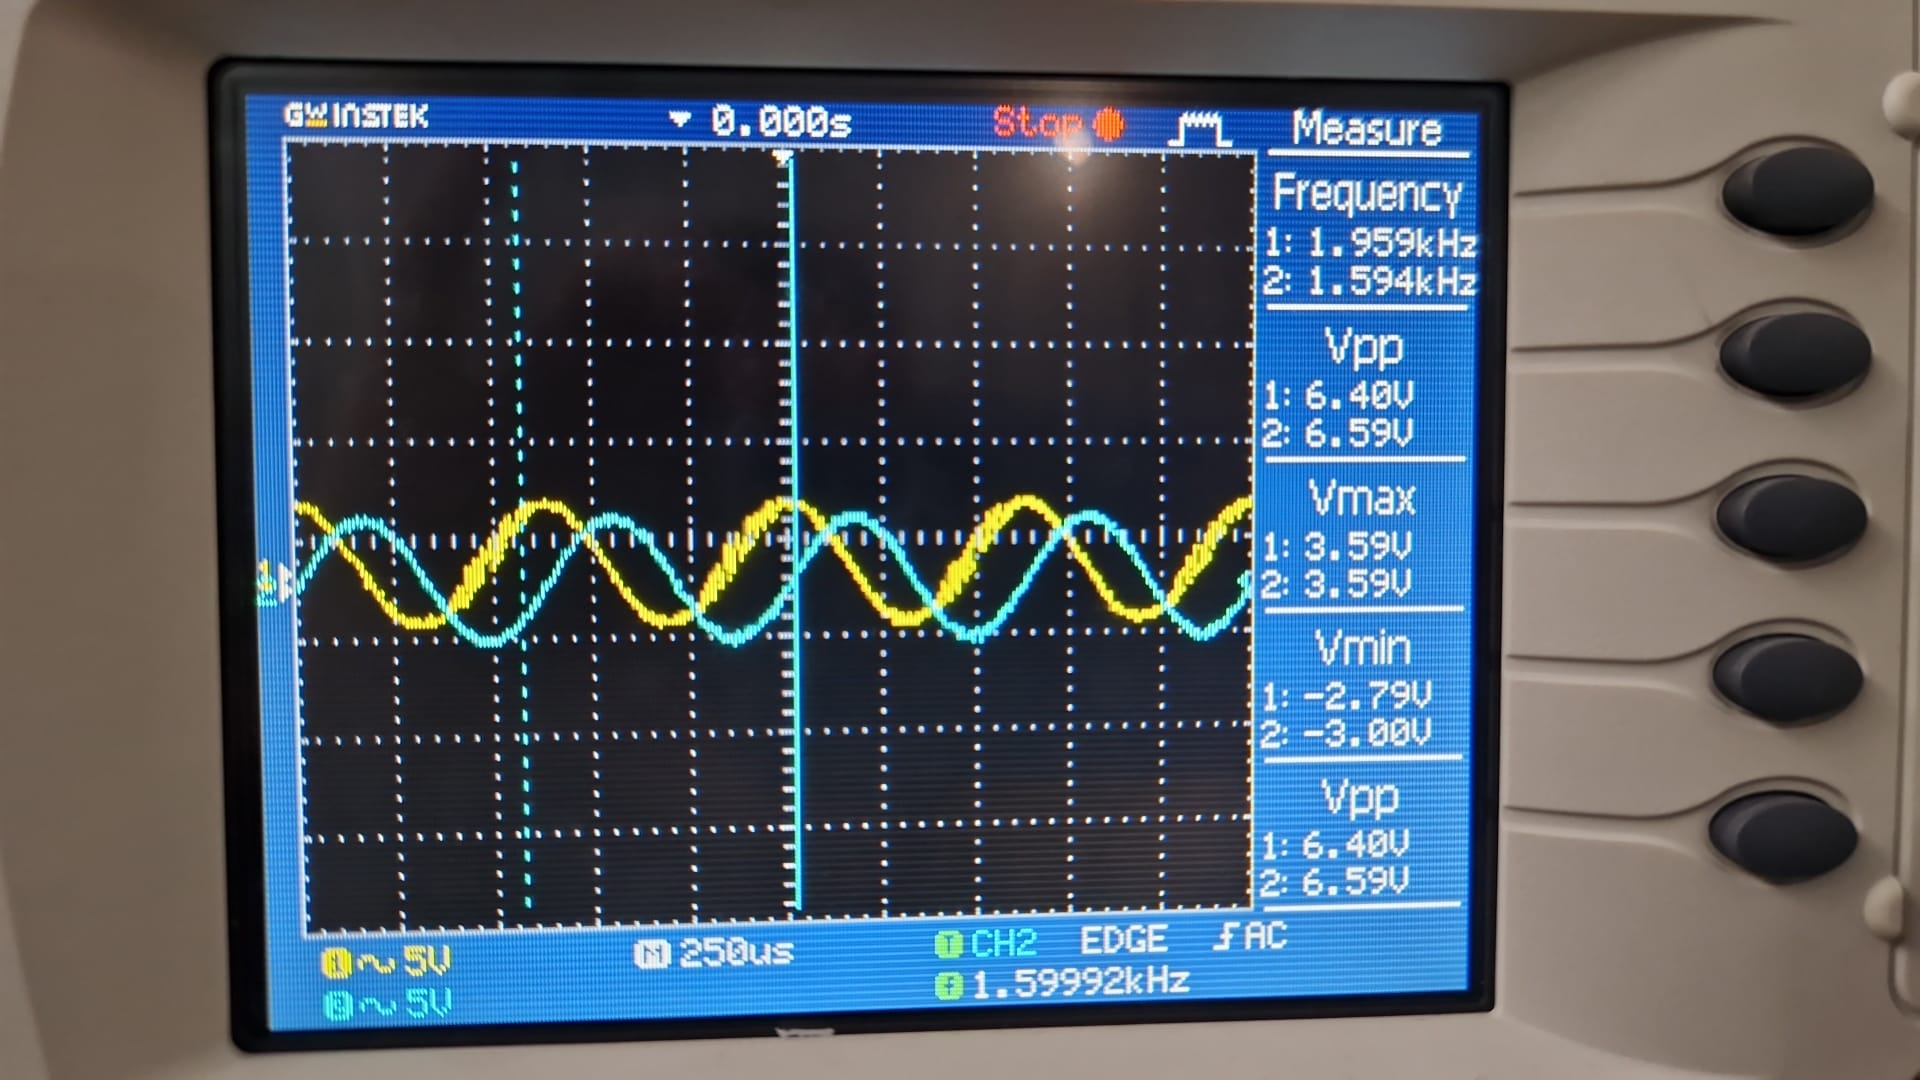
\includegraphics[width=1\linewidth]{assets/p2-exp-1.6.png}
        \caption{$1.6kHz$ Input signal}
        \label{fig:p2-exp-1.6}
    \end{minipage}%
    \begin{minipage}{.4\textwidth}
        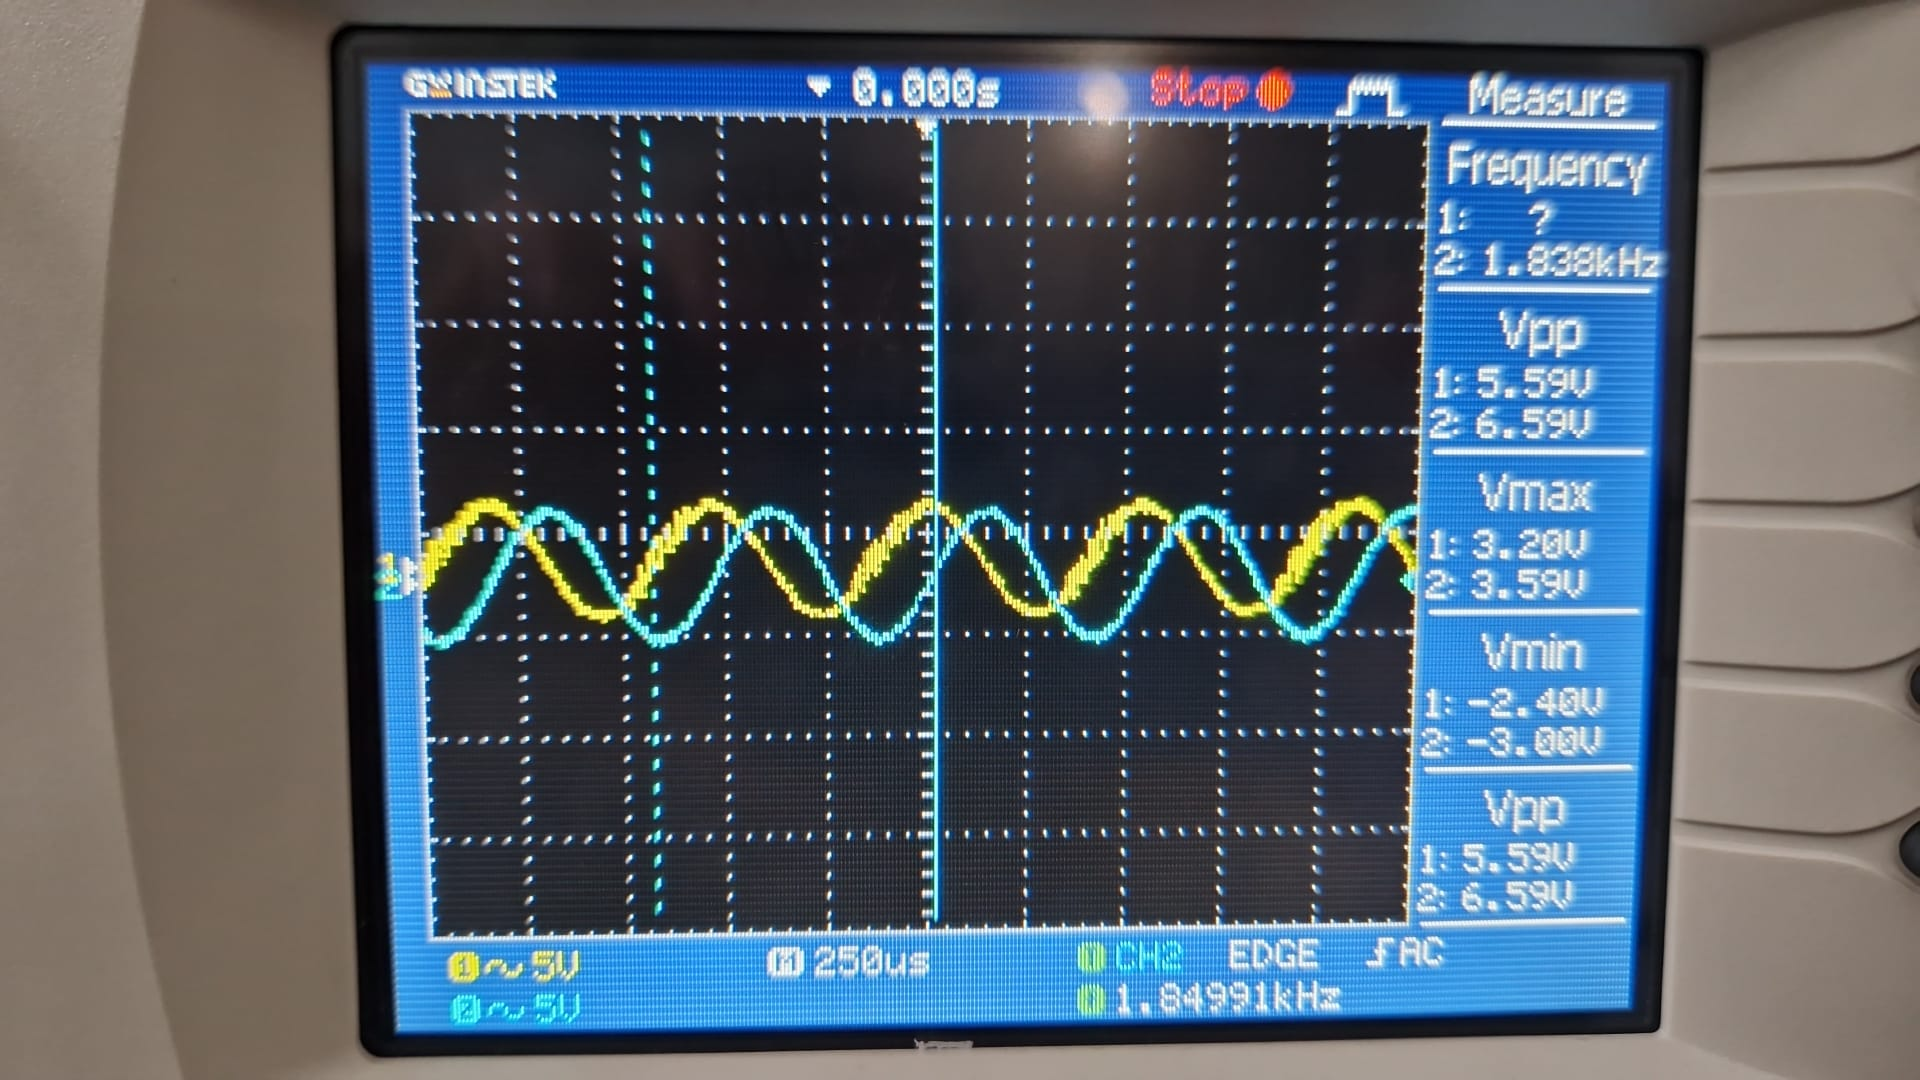
\includegraphics[width=1\linewidth]{assets/p2-exp-1.85.png}
        \caption{$1.85Hz$ Input signal}
        \label{fig:p2-exp-1.85}
    \end{minipage}
\end{figure}

\begin{itemize}
    \item \textbf{Frequency @ 100Hz:} The input and output voltages were plotted simultaneously. In the observed results, it was observed that at this low frequency, the output of the op-amp closely follows the input signal and the phase difference of the signal is minimum.
    \newpage
    \thispagestyle{plain}
    \item \textbf{Increasing the Frequency:} As the frequency increases, the output signal starts to lag behind the input signal. This is due to the phase shifts introduced by the op-amp at higher frequencies. The amplitude of the output signal also decreases as the frequency increases, indicating a drop in gain as the op-amp bandwidth is exceeded.
    \item The op-amp circuit performed as expected at low frequencies. The output signal largely followed the input signal and the gain remained constant.
    \item As the frequency increased, a significant phase shift in the output signal was observed due to the internal capacitances and feedback delays of the op-amp. The amplitude also decreased significantly. This was a typical gain reduction that occurs when the frequency limits of the op-amp are approached. The experiment confirmed that at high frequencies the op-amp has limited performance and the signal degrades when the bandwidth is exceeded.
    \item According to the comparison between the Frequency Response Analysis simulation and the laboratory experiments, the op-amp circuit provided a stable gain at low frequencies as expected. However, as the frequency increases, especially when it approaches 1 kHz, a gain drop was observed in both simulation and experiment. This is due to phase shifts and decreases in amplitude caused by exceeding the bandwidth of the op-amp. The experimental results are in agreement with the theoretical analyses, showing a difference in gain of about $10\%$ with small deviations such as component tolerances.
\end{itemize}

\newpage{}
\thispagestyle{plain}

\section{Non-Inverting Amplifier Design}

\subsection{Theoretical Analysis}

For non-inverting amplifier design, we need to calculate the resistor values for the desired gain. The formula for calculating the resistor values is given below:

\begin{align*}
    4 = 1 + \frac{R_{f}}{R_{1}} &\Rightarrow \frac{R_{f}}{R_{1}} = 3 \\
    R_{f} &= 3k\Omega, R_{1} = 1k\Omega
\end{align*}

\begin{figure}[h]
    \centering
    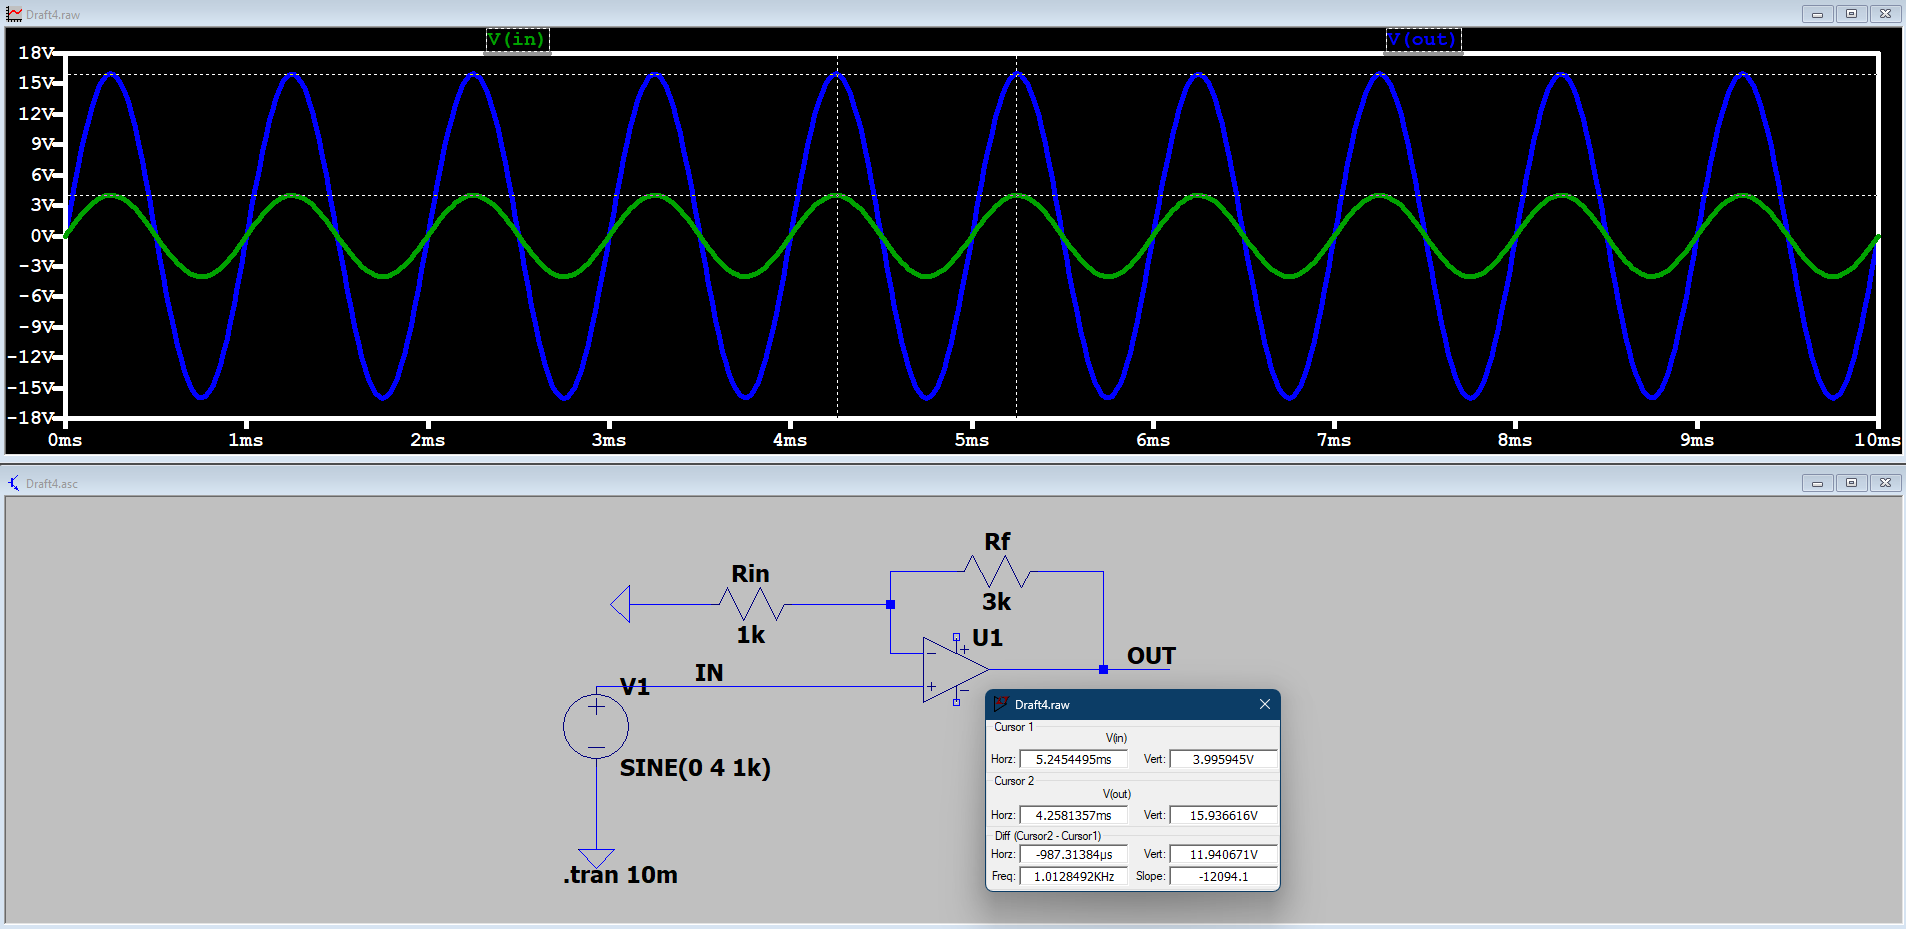
\includegraphics[width=0.8\textwidth]{assets/a4_design.png}
    \caption{Non-Inverting Amplifier Circuit @ 4V1kHz}
    \label{fig:non-inverting-amplifier-circuit-4v}
\end{figure}

\begin{figure}[h]
    \centering
    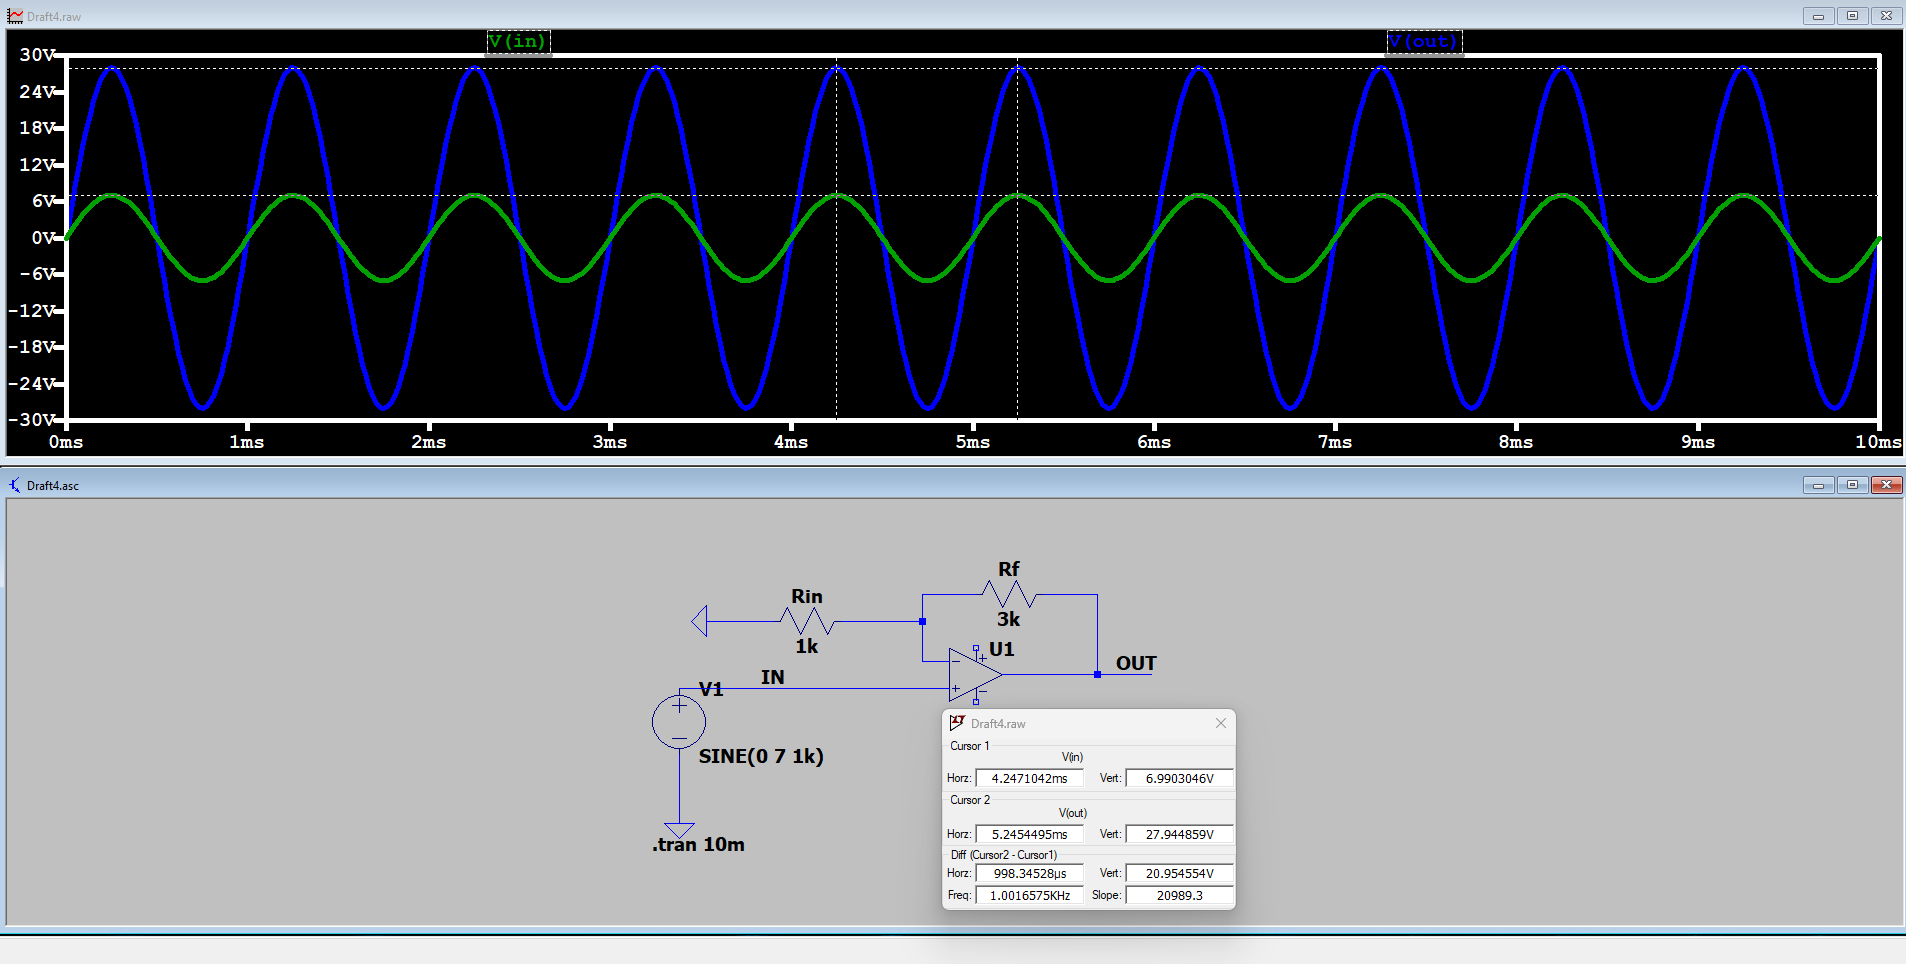
\includegraphics[width=0.8\textwidth]{assets/7_design.png}
    \caption{Non-Inverting Amplifier Circuit @ 7V1kHz}
    \label{fig:non-inverting-amplifier-circuit-7v}
\end{figure}

As we increase the voltage, the output voltage also increases. This is because the gain of the circuit is $4$.

\newpage
\thispagestyle{plain}

\subsection{Experimental Analysis}

To verify the theoretical results, we built the same circuit on a breadboard and measured the input and output voltages using an oscilloscope.

\begin{figure}[h]
    \centering
    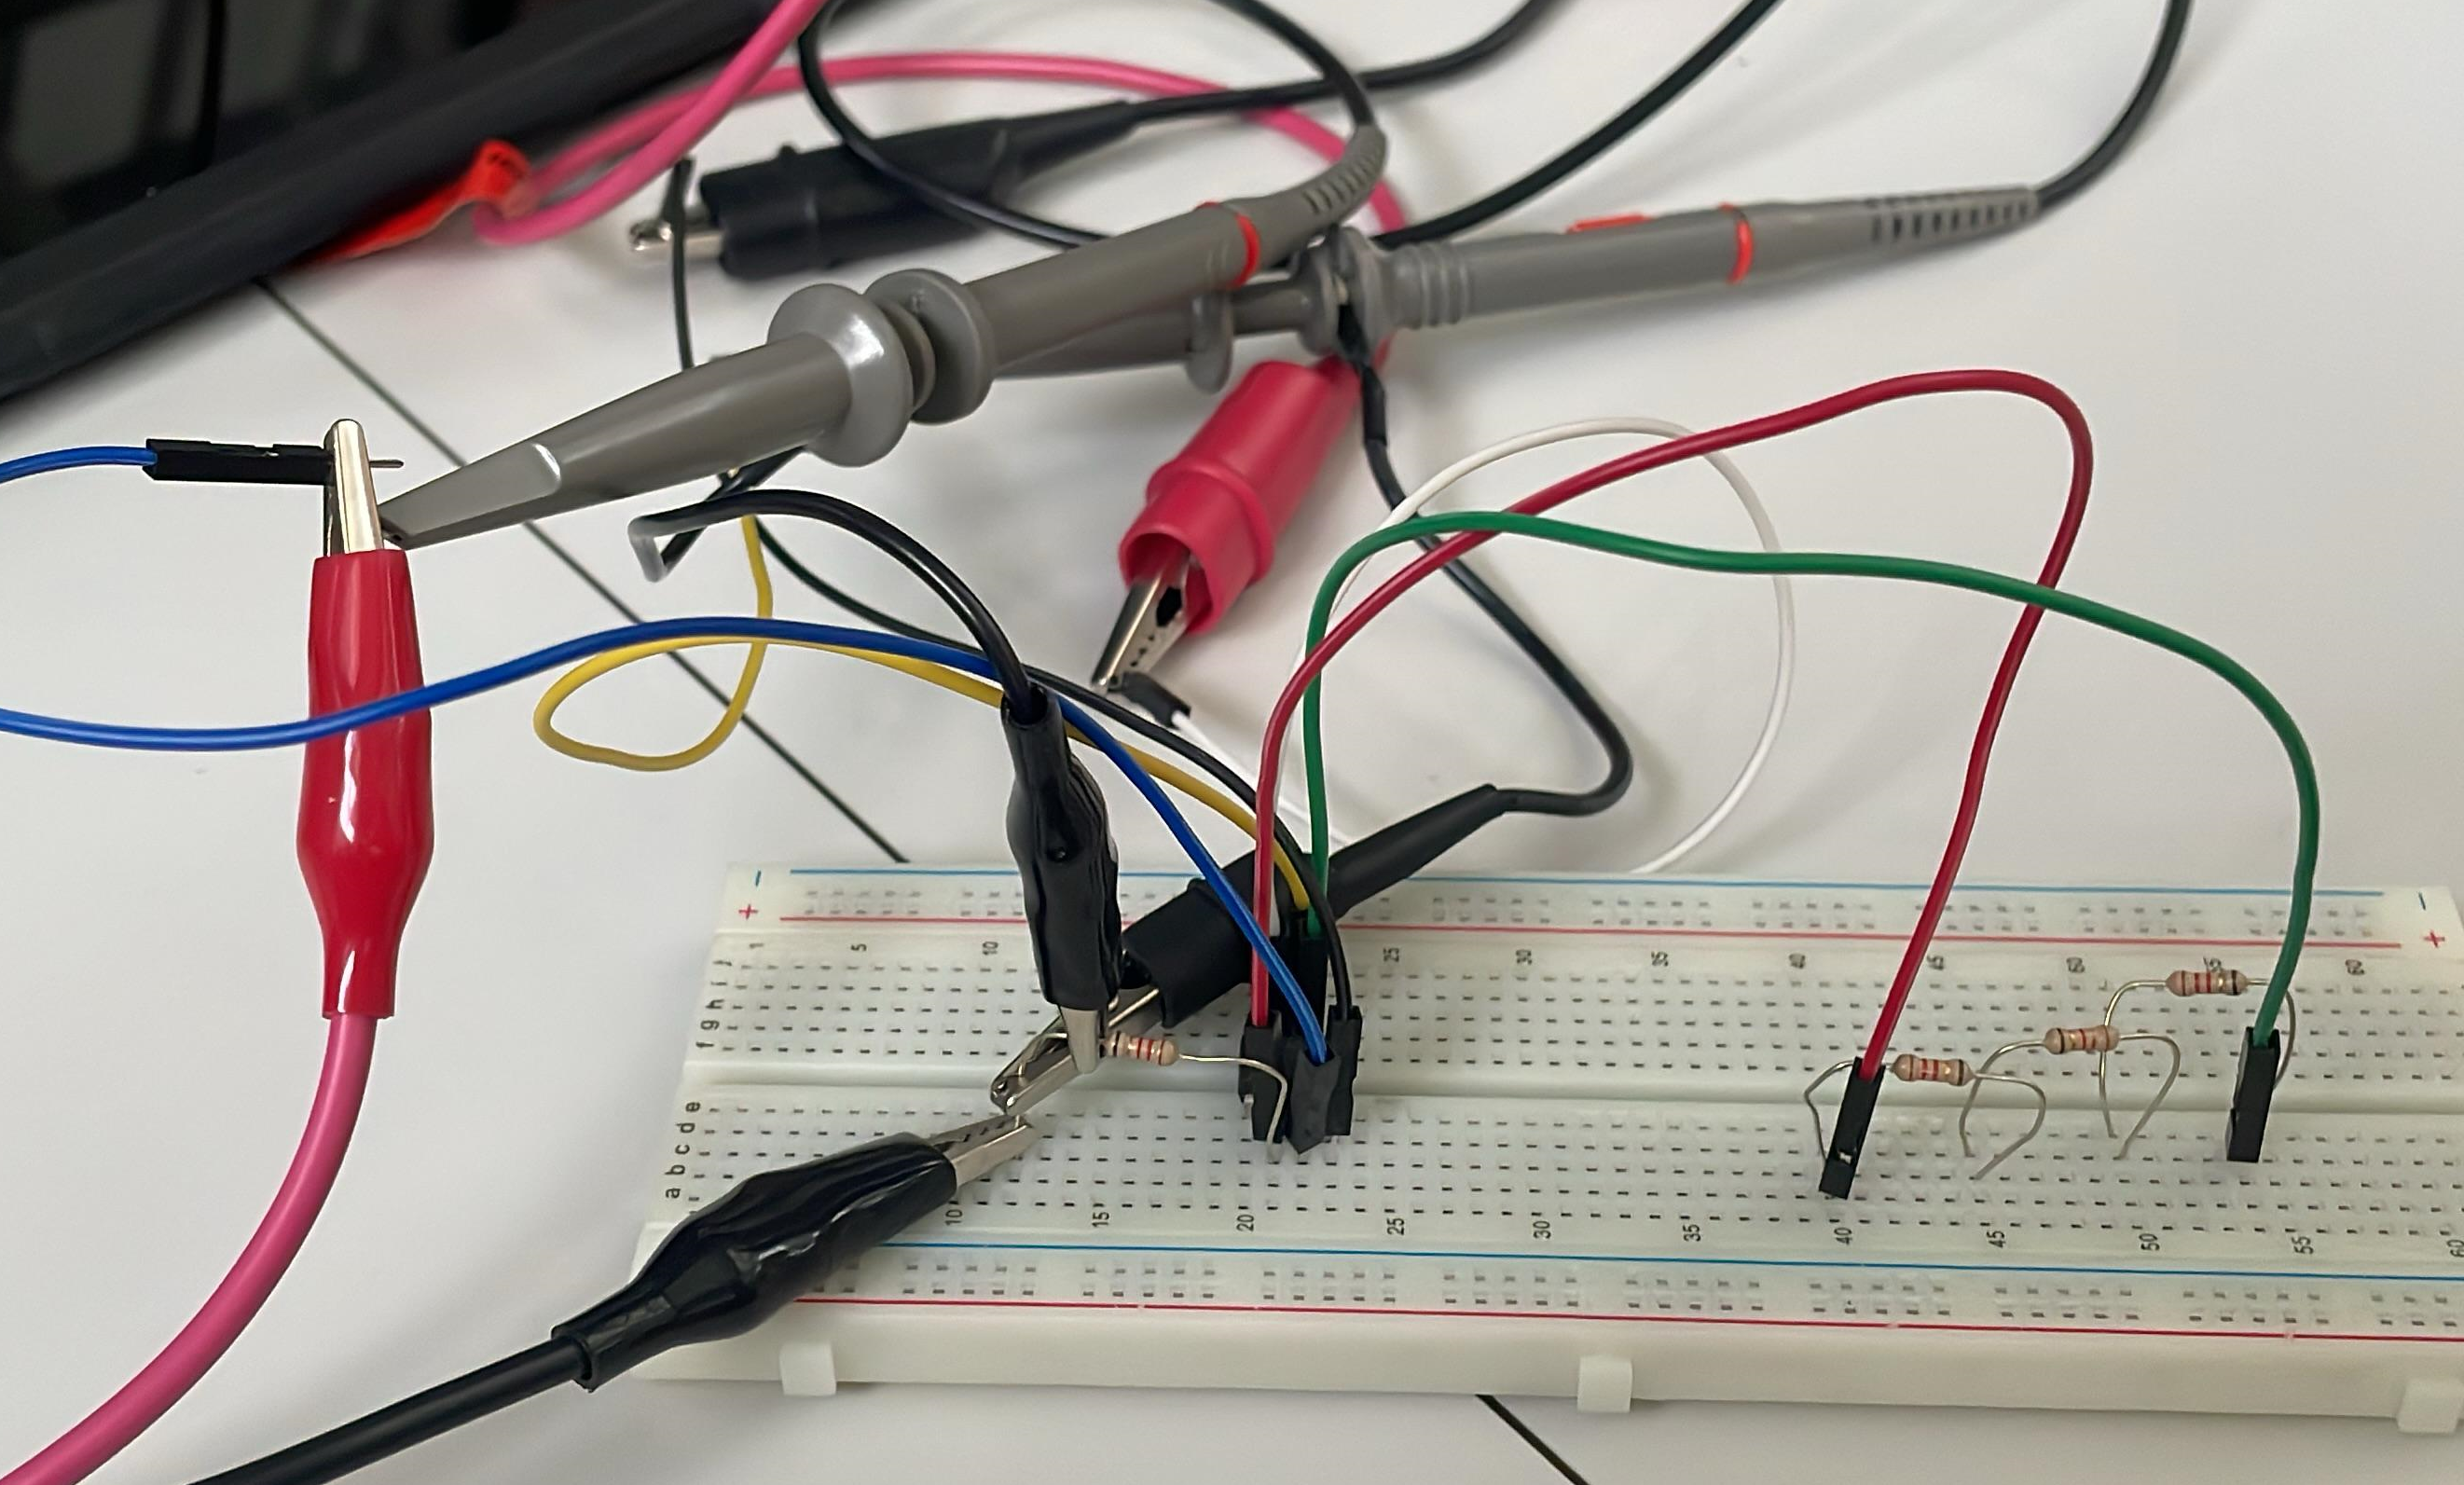
\includegraphics[width=0.8\textwidth]{assets/p3-circuit.png}
    \caption{Experiment Circuit}
    \label{fig:p3-circuit}
|\end{figure}

\begin{figure}[h]
    \centering
    \begin{minipage}{.4\textwidth}
        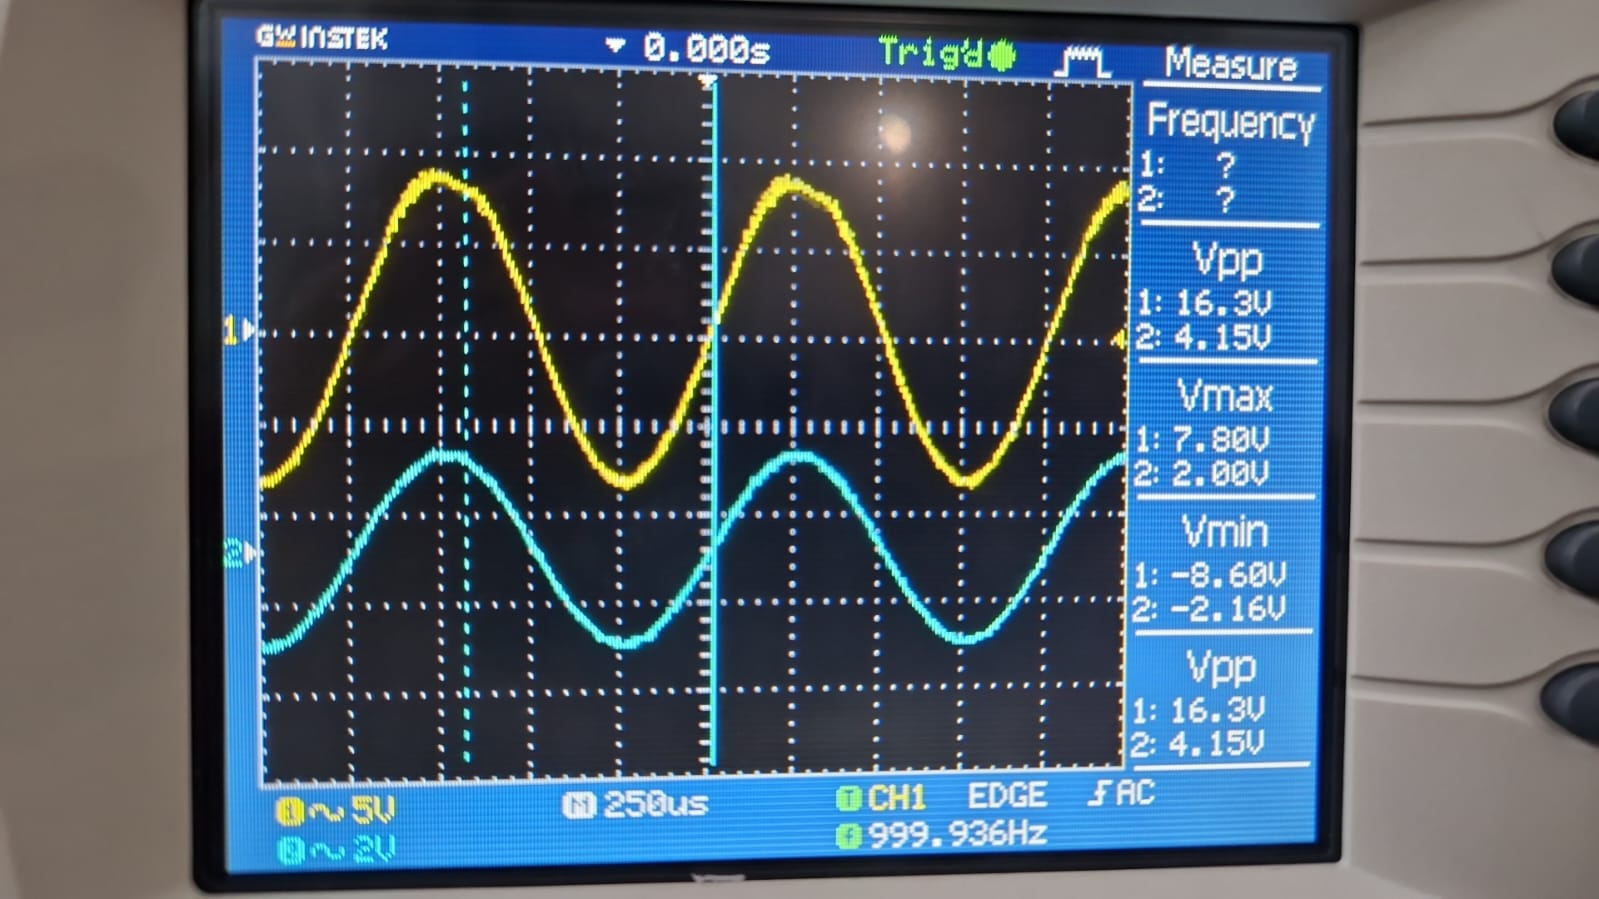
\includegraphics[width=1\linewidth]{assets/p3-exp-4.png}
        \caption{$4V_{pp}$ Input signal}
        \label{fig:p3-exp-4}
    \end{minipage}%
    \begin{minipage}{.4\textwidth}
        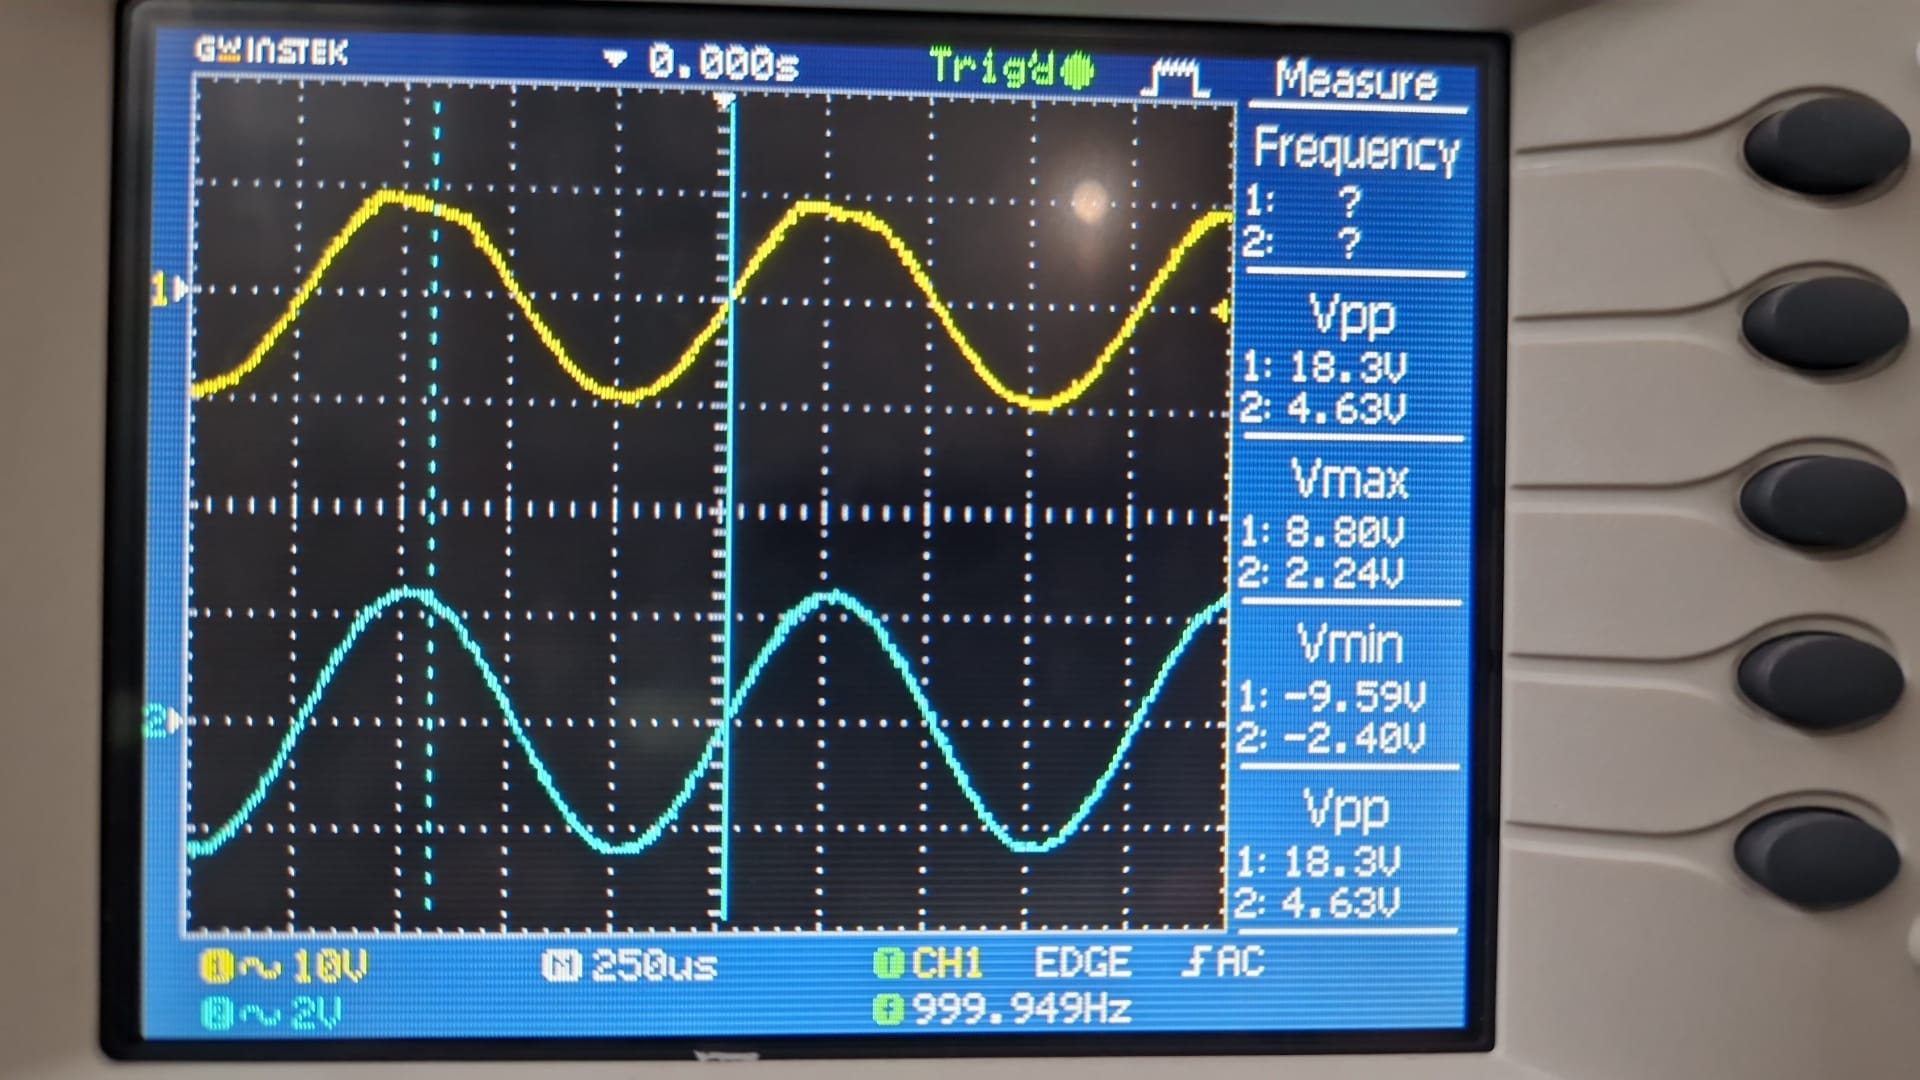
\includegraphics[width=1\linewidth]{assets/p3-exp-4.5.png}
        \caption{$4.5V_{pp}$ Input signal}
        \label{fig:p3-exp-4.5}
    \end{minipage}
    \begin{minipage}{.4\textwidth}
        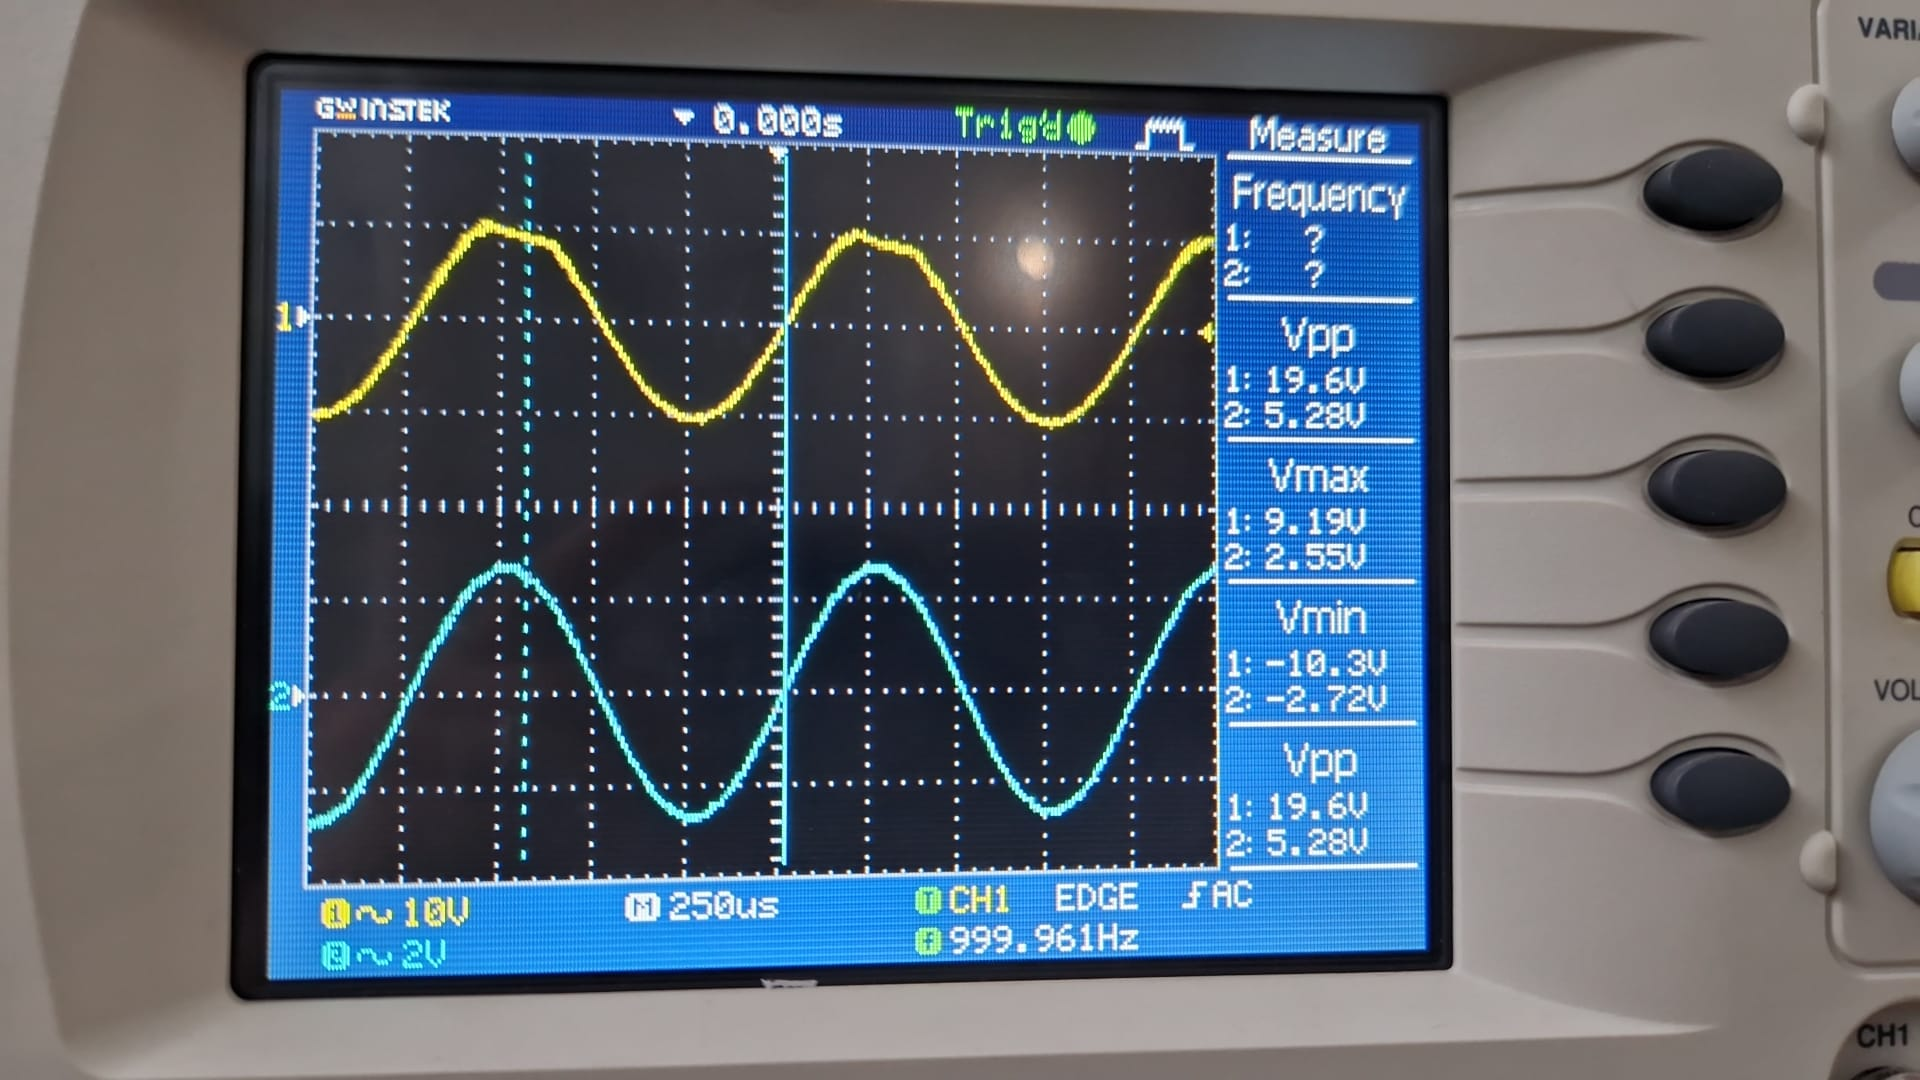
\includegraphics[width=1\linewidth]{assets/p3-exp-5.png}
        \caption{$5V_{pp}$ Input signal}
        \label{fig:p3-exp-5}
    \end{minipage}%
    \begin{minipage}{.4\textwidth}
        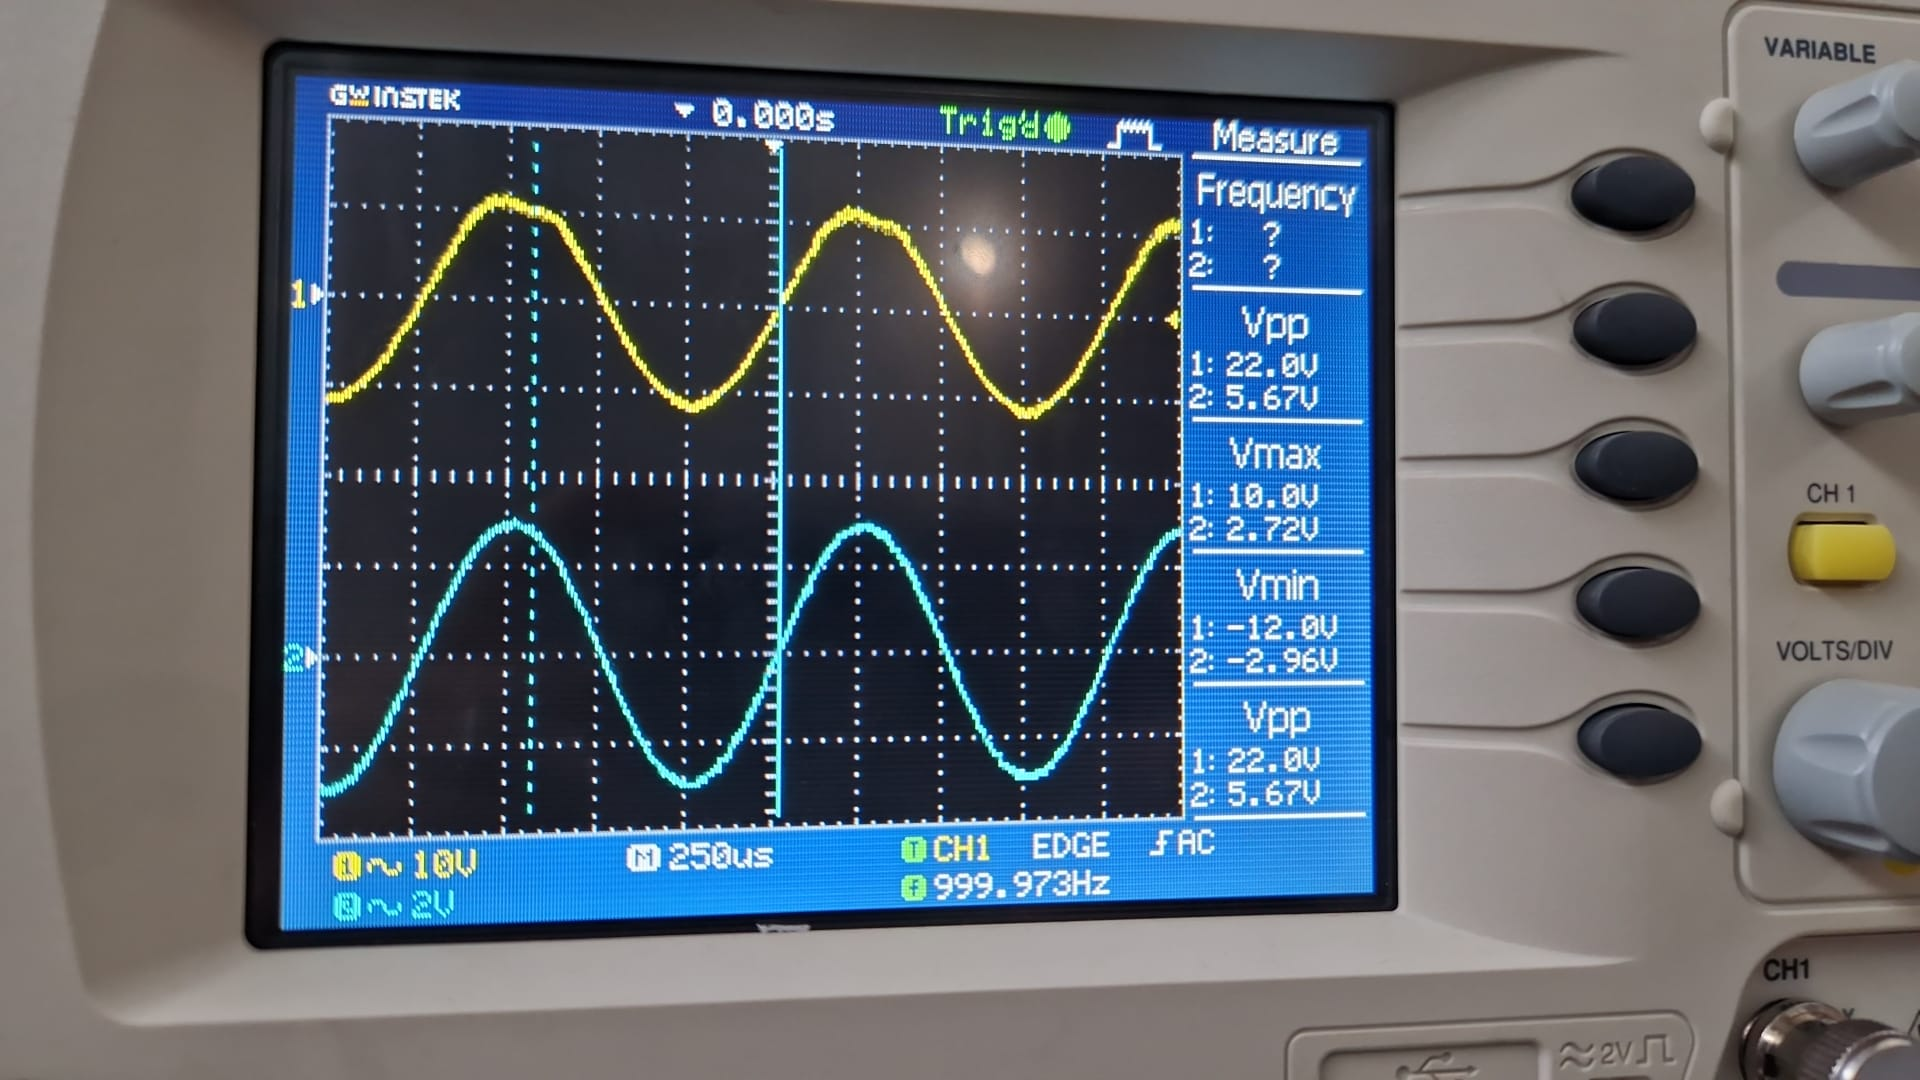
\includegraphics[width=1\linewidth]{assets/p3-exp-5.5.png}
        \caption{$5.5V_{pp}$ Input signal}
        \label{fig:p3-exp-5.5}
    \end{minipage}
\end{figure}

\newpage
\thispagestyle{plain}

\begin{figure}[h]
    \centering
    \begin{minipage}{.4\textwidth}
        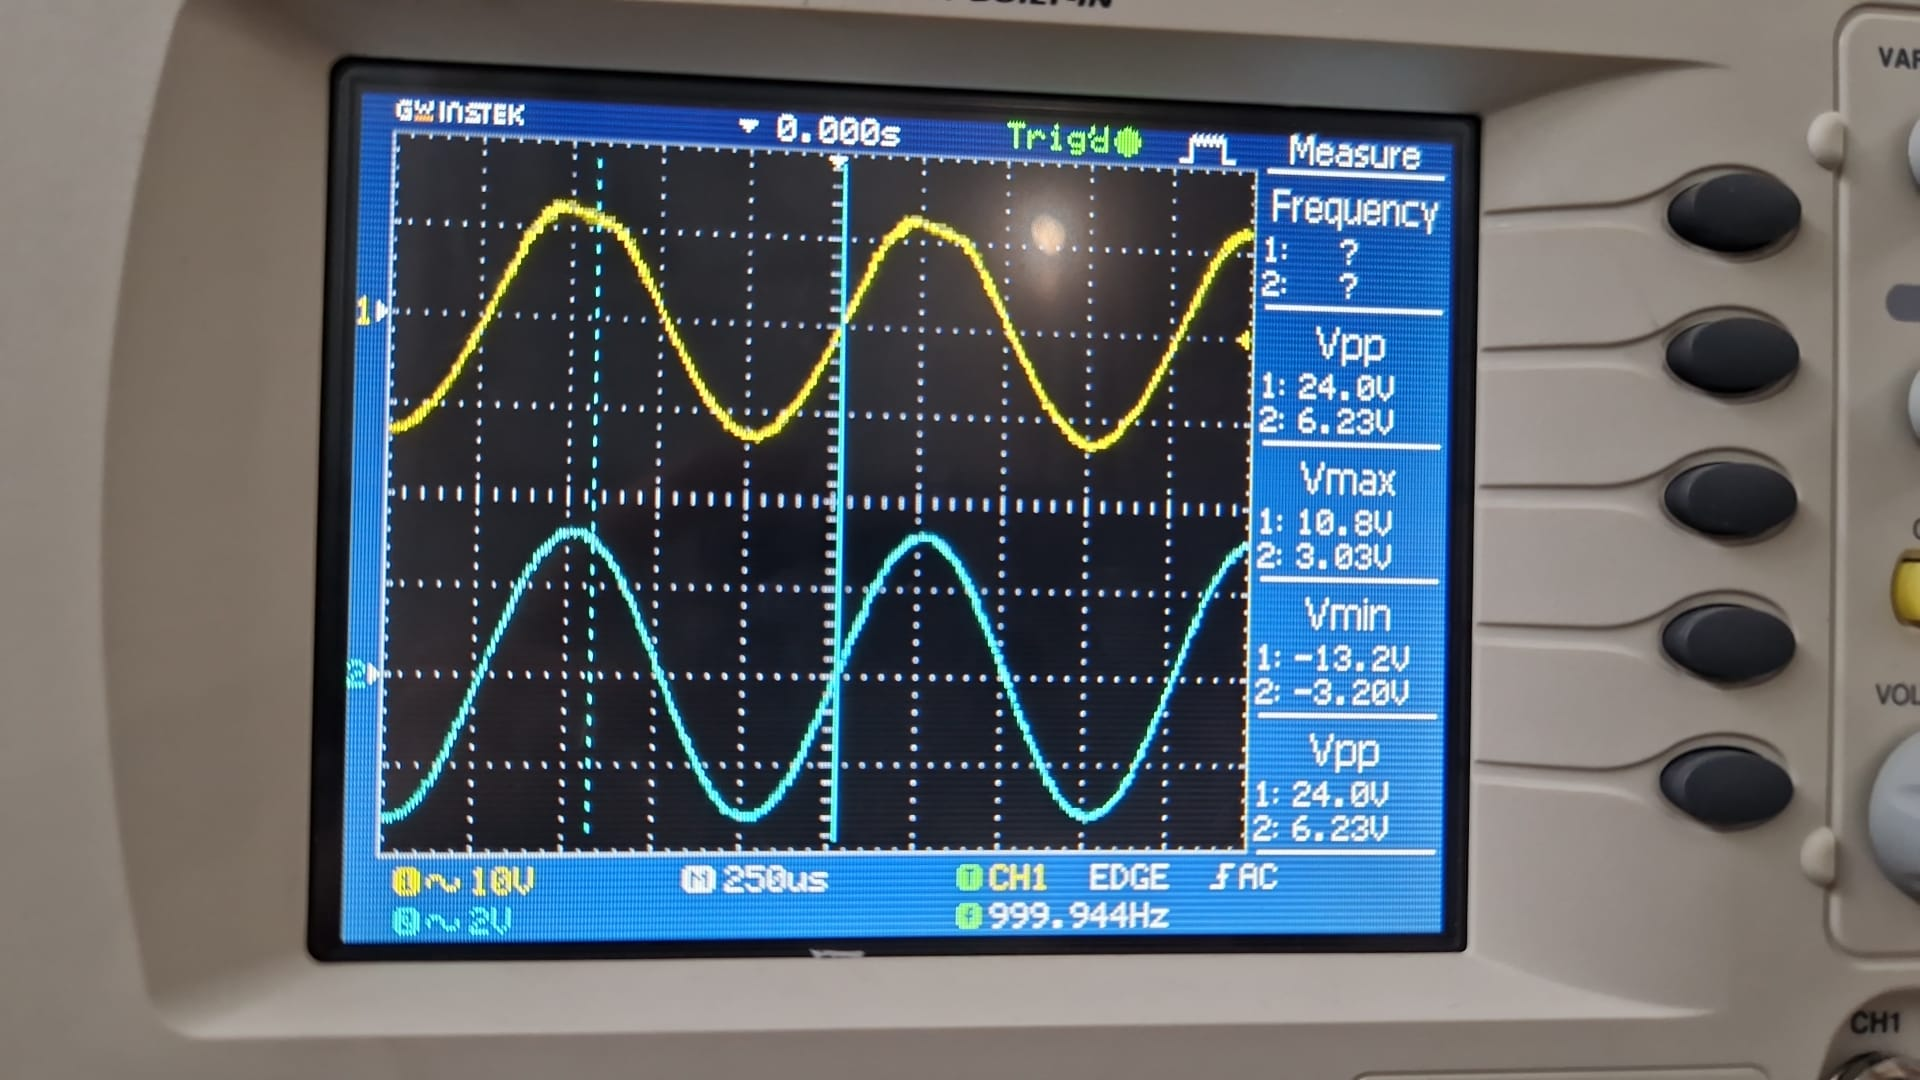
\includegraphics[width=1\linewidth]{assets/p3-exp-6.png}
        \caption{$6V_{pp}$ Input signal}
        \label{fig:p3-exp-6}
    \end{minipage}%
    \begin{minipage}{.4\textwidth}
        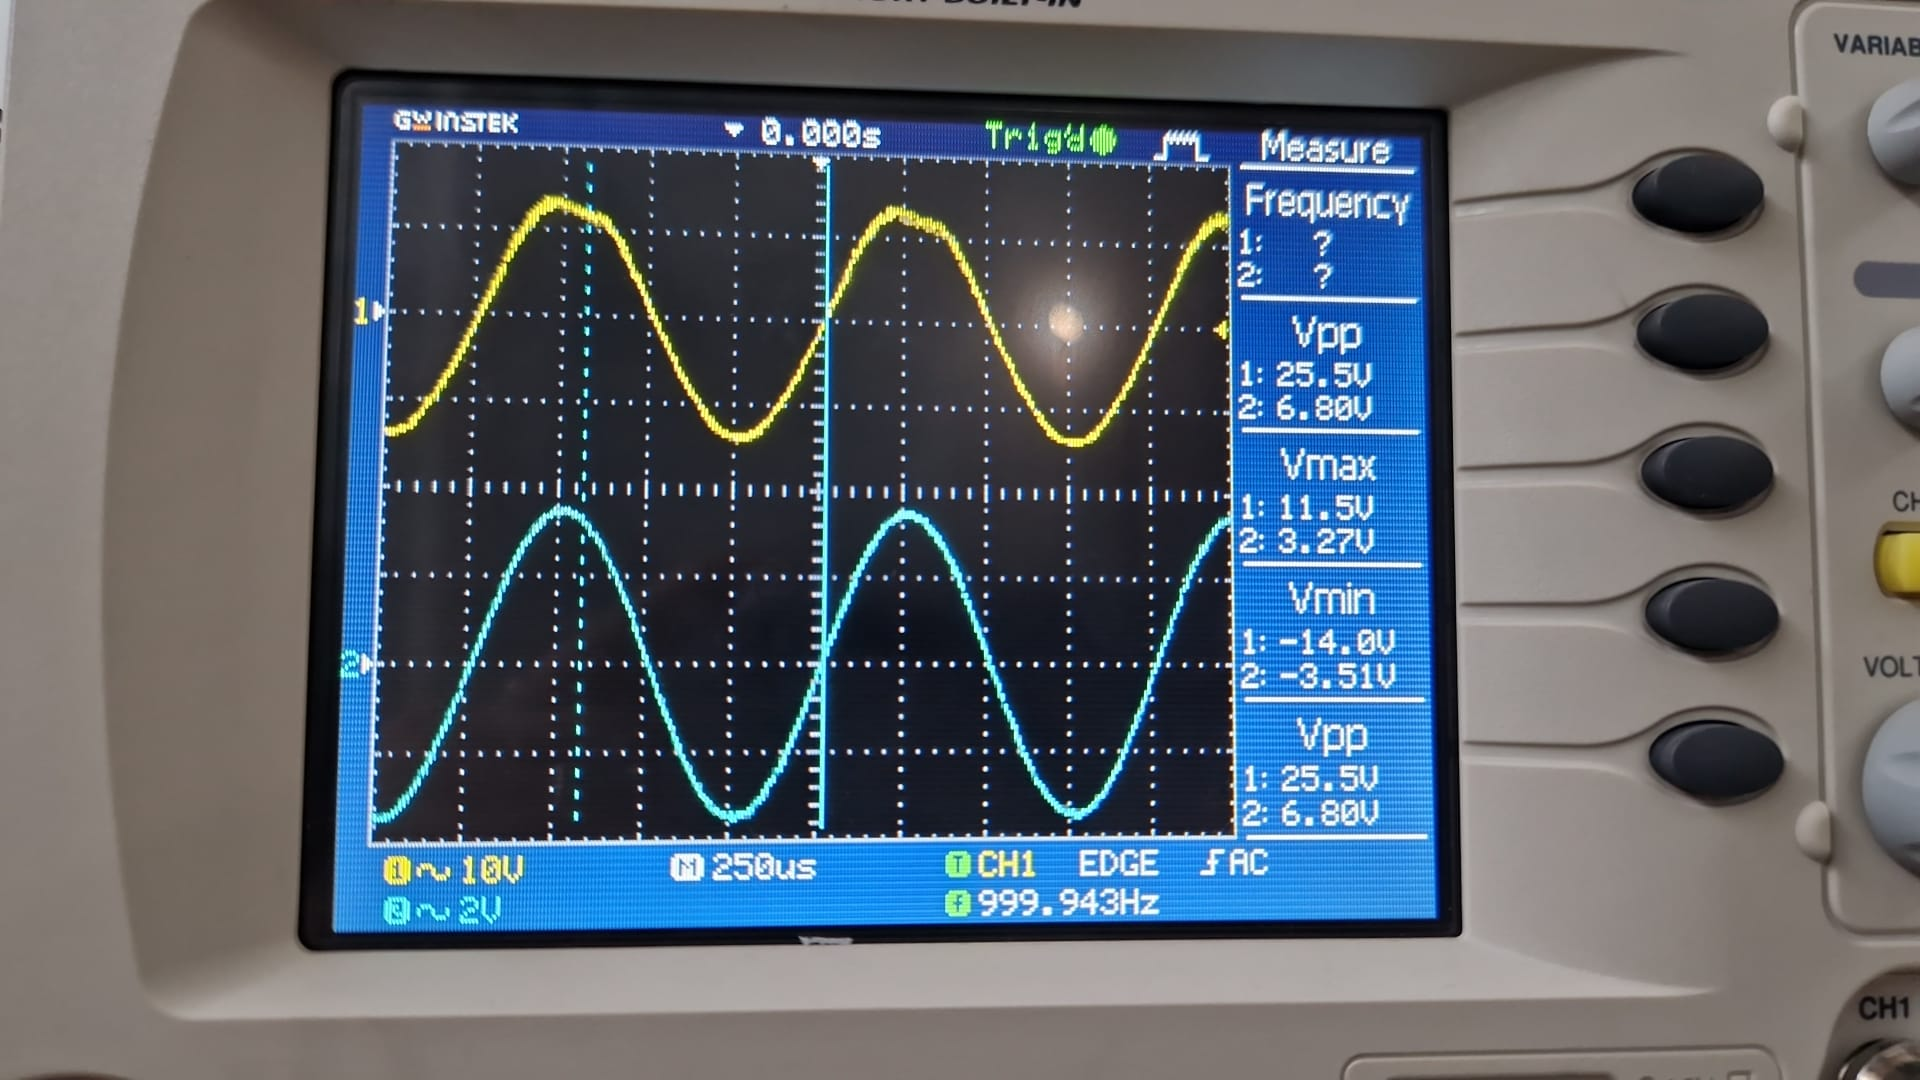
\includegraphics[width=1\linewidth]{assets/p3-exp-6.5.png}
        \caption{$6.5V_{pp}$ Input signal}
        \label{fig:p3-exp-6.5}
    \end{minipage}
    \begin{minipage}{.4\textwidth}
        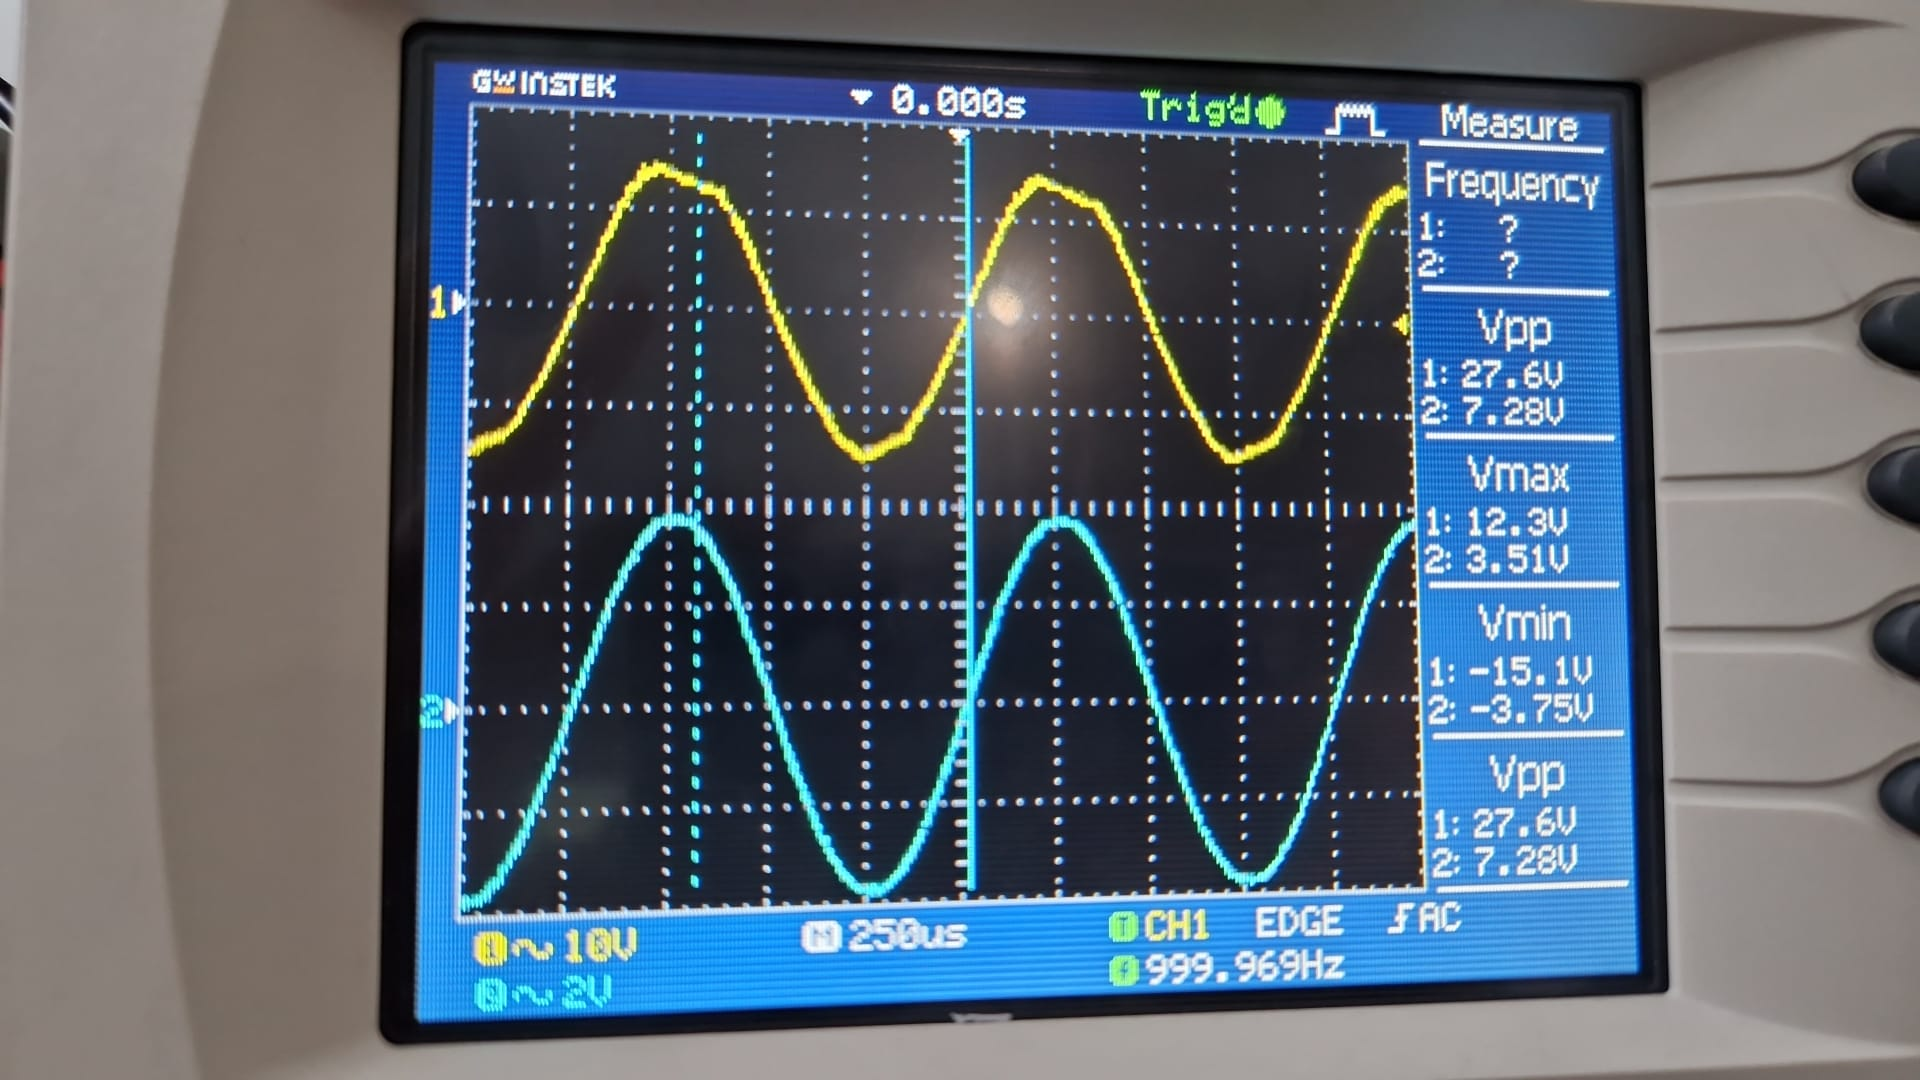
\includegraphics[width=1\linewidth]{assets/p3-exp-7.png}
        \caption{$7V_{pp}$ Input signal}
        \label{fig:p3-exp-7}
    \end{minipage}
\end{figure}

Yellow lines represent the output voltage, and the blue lines represent the input voltage. The gain of the voltage results in a proportional increase in the output voltage accordingly. There is very little change in the values, however, that is expected due to the tolerances of the resistors and probes used in the circuit. Input voltage ($V_{in}$) and output voltage ($V_{out} = 4V_{in}$) are in agreement with the theoretical analysis.
